\documentclass[12pt,a4paper]{report}

% ─── Packages ────────────────────────────────────────────────────────────────
\usepackage[a4paper, margin=2.5cm]{geometry}
\usepackage[T1]{fontenc}
\usepackage[utf8]{inputenc}
\usepackage{lmodern}
\usepackage{microtype}
\usepackage{xcolor}
\usepackage{graphicx}
\usepackage{booktabs}
\usepackage{longtable}
\usepackage{array}
\usepackage{tabularx}
\usepackage{multirow}
\usepackage{enumitem}
\usepackage{listings}
\usepackage{fancyhdr}
\usepackage{titlesec}
\usepackage{tocloft}
\usepackage{hyperref}
\usepackage{amsmath}
\usepackage{amssymb}
\usepackage{tikz}
\usepackage{pgf}
\usetikzlibrary{shapes.geometric, arrows.meta, positioning, fit, backgrounds, calc}
\usepackage{mdframed}
\usepackage{tcolorbox}
\tcbuselibrary{skins, breakable}
\usepackage{fontawesome5}
\usepackage{setspace}
\usepackage{caption}
\usepackage{subcaption}

% ─── Colour Palette ──────────────────────────────────────────────────────────
\definecolor{primary}{HTML}{1E3A5F}
\definecolor{secondary}{HTML}{2E86AB}
\definecolor{accent}{HTML}{E84855}
\definecolor{success}{HTML}{3BB273}
\definecolor{warning}{HTML}{F4A261}
\definecolor{lightgray}{HTML}{F5F5F5}
\definecolor{darkgray}{HTML}{333333}
\definecolor{codebg}{HTML}{1E1E2E}
\definecolor{codetext}{HTML}{CDD6F4}
\definecolor{p1red}{HTML}{C0392B}
\definecolor{p2orange}{HTML}{E67E22}
\definecolor{p3blue}{HTML}{2980B9}
\definecolor{p4green}{HTML}{27AE60}

% ─── Hyperref Setup ──────────────────────────────────────────────────────────
\hypersetup{
  colorlinks=true,
  linkcolor=primary,
  urlcolor=secondary,
  citecolor=accent,
  pdftitle={White Box Testing Document -- Stockly},
  pdfauthor={Stockly Engineering},
  pdfsubject={White Box Testing},
}

% ─── Header / Footer ─────────────────────────────────────────────────────────
\pagestyle{fancy}
\fancyhf{}
\fancyhead[L]{\small\color{primary}\textbf{Stockly} -- White Box Testing}
\fancyhead[R]{\small\color{darkgray}v2.0.1}
\fancyfoot[C]{\small\color{darkgray}\thepage}
\renewcommand{\headrulewidth}{0.4pt}
\renewcommand{\footrulewidth}{0.4pt}

% ─── Section Styling ─────────────────────────────────────────────────────────
\titleformat{\chapter}[display]
  {\normalfont\huge\bfseries\color{primary}}
  {\chaptertitlename\ \thechapter}{20pt}{\Huge}
\titleformat{\section}
  {\normalfont\Large\bfseries\color{primary}}
  {\thesection}{1em}{}
\titleformat{\subsection}
  {\normalfont\large\bfseries\color{secondary}}
  {\thesubsection}{1em}{}
\titleformat{\subsubsection}
  {\normalfont\normalsize\bfseries\color{darkgray}}
  {\thesubsubsection}{1em}{}

% ─── Code Listing Style ──────────────────────────────────────────────────────
\lstdefinestyle{codestyle}{
  backgroundcolor=\color{codebg},
  basicstyle=\ttfamily\small\color{codetext},
  keywordstyle=\color{accent}\bfseries,
  commentstyle=\color{success}\itshape,
  stringstyle=\color{warning},
  breaklines=true,
  frame=single,
  rulecolor=\color{secondary},
  numbers=left,
  numberstyle=\tiny\color{darkgray},
  tabsize=2,
  showstringspaces=false,
}
\lstset{style=codestyle}

% ─── Custom Boxes ────────────────────────────────────────────────────────────
\tcbset{
  testbox/.style={
    enhanced, breakable,
    colback=lightgray, colframe=secondary,
    fonttitle=\bfseries\color{white},
    coltitle=white, attach boxed title to top left,
    boxed title style={colback=secondary, rounded corners},
    rounded corners, drop shadow,
  },
  criticalbox/.style={
    enhanced, breakable,
    colback=red!5, colframe=p1red,
    fonttitle=\bfseries\color{white},
    coltitle=white, attach boxed title to top left,
    boxed title style={colback=p1red, rounded corners},
    rounded corners,
  },
  infobox/.style={
    enhanced, breakable,
    colback=blue!5, colframe=primary,
    fonttitle=\bfseries\color{white},
    coltitle=white, attach boxed title to top left,
    boxed title style={colback=primary, rounded corners},
    rounded corners,
  },
  warningbox/.style={
    enhanced, breakable,
    colback=orange!8, colframe=warning,
    fonttitle=\bfseries\color{white},
    coltitle=white, attach boxed title to top left,
    boxed title style={colback=warning, rounded corners},
    rounded corners,
  },
}

% ─── TikZ Flowchart Styles ───────────────────────────────────────────────────
\tikzset{
  startstop/.style={
    rectangle, rounded corners=8pt,
    minimum width=3cm, minimum height=0.9cm,
    text centered, draw=primary, very thick,
    fill=primary!15, font=\small\bfseries,
  },
  process/.style={
    rectangle,
    minimum width=3.5cm, minimum height=0.9cm,
    text centered, draw=secondary, thick,
    fill=secondary!10, font=\small,
  },
  decision/.style={
    diamond, aspect=2.2,
    minimum width=3.5cm, minimum height=0.9cm,
    text centered, draw=accent, thick,
    fill=accent!10, font=\small,
  },
  io/.style={
    trapezium, trapezium left angle=70, trapezium right angle=110,
    minimum width=3cm, minimum height=0.9cm,
    text centered, draw=success, thick,
    fill=success!10, font=\small,
  },
  terminal/.style={
    rectangle, rounded corners=15pt,
    minimum width=2.5cm, minimum height=0.9cm,
    text centered, draw=accent, very thick,
    fill=accent!20, font=\small\bfseries,
  },
  arrow/.style={-{Stealth[length=6pt]}, thick, color=darkgray},
  yes/.style={font=\small\color{success}\bfseries},
  no/.style={font=\small\color{accent}\bfseries},
}

% ─── Misc Helpers ────────────────────────────────────────────────────────────
\newcommand{\testid}[1]{\texttt{\textbf{\color{secondary}#1}}}
\newcommand{\branch}[1]{\texttt{\color{accent}#1}}
\newcommand{\pone}{\textbf{\color{p1red}P1}}
\newcommand{\ptwo}{\textbf{\color{p2orange}P2}}
\newcommand{\pthree}{\textbf{\color{p3blue}P3}}
\newcommand{\pfour}{\textbf{\color{p4green}P4}}

\setlength{\parskip}{6pt}
\setlength{\parindent}{0pt}

% ─────────────────────────────────────────────────────────────────────────────
\begin{document}
% ─────────────────────────────────────────────────────────────────────────────

% ══════════════════════════════════════════════════════════════════════════════
%  TITLE PAGE
% ══════════════════════════════════════════════════════════════════════════════
\begin{titlepage}
  \pagecolor{primary}
  \color{white}
  \centering
  \vspace*{3cm}

  {\fontsize{14}{18}\selectfont\texttt{STOCKLY ENGINEERING}}\\[0.5cm]
  \rule{12cm}{1pt}\\[0.8cm]
  {\fontsize{36}{44}\selectfont\bfseries White Box\\[0.3cm]Testing Document}\\[0.8cm]
  \rule{12cm}{1pt}\\[1cm]

  {\Large\itshape Inventory \& Supply Chain Management System}\\[2cm]

  \begin{tabular}{rl}
    \textbf{Project:}   & Stockly v2.0.1 \\[4pt]
    \textbf{Stack:}     & Next.js 16, TypeScript, Prisma, MongoDB \\[4pt]
    \textbf{Date:}      & April 1, 2026 \\[4pt]
    \textbf{Modules:}   & 10 \\[4pt]
    \textbf{Test Cases:}& 107 \\[4pt]
    \textbf{Coverage Target:} & 85\% Statements / 90\% Branches \\
  \end{tabular}

  \vfill
  {\small\color{white!70} Generated for internal engineering use only.}
\end{titlepage}
\pagecolor{white}\color{black}

% ══════════════════════════════════════════════════════════════════════════════
%  TABLE OF CONTENTS
% ══════════════════════════════════════════════════════════════════════════════
\tableofcontents
\newpage


% ══════════════════════════════════════════════════════════════════════════════
\chapter{Introduction to White Box Testing}
% ══════════════════════════════════════════════════════════════════════════════

\begin{tcolorbox}[infobox, title={What is White Box Testing?}]
White box testing (also called \textbf{structural testing}, \textbf{glass-box testing}, or
\textbf{clear-box testing}) is a software testing technique that examines the \emph{internal}
logic, code paths, branches, loops, and data flows of an application --- not just its external
behaviour. Unlike black-box testing, white box testing requires the tester to have full
knowledge of the source code.
\end{tcolorbox}

\section{Key Goals}

\begin{itemize}[leftmargin=1.5em]
  \item Achieve \textbf{100\% statement coverage} --- every line of code is executed at least once.
  \item Achieve \textbf{100\% branch coverage} --- every \texttt{if}/\texttt{else} branch is tested.
  \item Achieve \textbf{100\% path coverage} --- every unique execution path is tested.
  \item Validate all \texttt{catch} blocks are reachable and handled correctly.
  \item Verify all loops execute correctly for 0, 1, and $N$ iterations.
  \item Confirm data transformations produce mathematically correct results.
  \item Ensure security boundaries cannot be bypassed through internal logic.
\end{itemize}

\section{Types of White Box Testing Used}

\begin{enumerate}[leftmargin=1.5em]
  \item \textbf{Unit Testing} --- Testing individual functions in isolation.
  \item \textbf{Integration Testing} --- Testing how modules interact with each other.
  \item \textbf{Control Flow Testing} --- Testing all branches and decision points.
  \item \textbf{Data Flow Testing} --- Tracking how data is created, used, and destroyed.
  \item \textbf{Mutation Testing} --- Verifying tests catch intentional code bugs.
  \item \textbf{Boundary Value Analysis} --- Testing edge values at limits.
\end{enumerate}

\section{Priority Classification}

\begin{center}
\begin{tabular}{clp{9cm}}
  \toprule
  \textbf{Priority} & \textbf{Label} & \textbf{Meaning} \\
  \midrule
  \pone & Critical & Security, financial logic, auth guards. Must pass before any release. \\
  \ptwo & High     & Core business logic, stock management, role-based access. \\
  \pthree & Medium & Edge cases, format validation, confidence scores. \\
  \pfour & Low     & Informational, documentation-level tests. \\
  \bottomrule
\end{tabular}
\end{center}

% ══════════════════════════════════════════════════════════════════════════════
\chapter{Project Architecture Overview}
% ══════════════════════════════════════════════════════════════════════════════

\section{Technology Stack}

\begin{center}
\begin{tabularx}{\textwidth}{lX}
  \toprule
  \textbf{Layer} & \textbf{Technology} \\
  \midrule
  Framework    & Next.js 16 (App Router) \\
  Language     & TypeScript (strict mode) \\
  Database     & MongoDB via Prisma ORM 6.4 \\
  Auth         & JWT (\texttt{jsonwebtoken}) + \texttt{bcryptjs} \\
  Cache        & Redis / Upstash \\
  Payments     & Stripe \\
  Shipping     & Shippo \\
  Email        & Brevo (Sendinblue) + QStash queue \\
  Validation   & Zod schemas \\
  Monitoring   & Sentry \\
  \bottomrule
\end{tabularx}
\end{center}

\section{User Roles}

\begin{center}
\begin{tabular}{lp{10cm}}
  \toprule
  \textbf{Role} & \textbf{Access Level} \\
  \midrule
  \texttt{admin}    & Full system access \\
  \texttt{user}     & Standard product/order management \\
  \texttt{supplier} & View products they supply, view related orders \\
  \texttt{client}   & View their own orders and invoices \\
  \texttt{retailer} & Limited access (similar to client) \\
  \bottomrule
\end{tabular}
\end{center}

\section{Core Data Models}

\begin{center}
\begin{tabular}{ll}
  \toprule
  \textbf{Model} & \textbf{Purpose} \\
  \midrule
  \texttt{User}            & Authentication, roles, preferences \\
  \texttt{Product}         & Inventory items with \texttt{quantity} + \texttt{reservedQuantity} \\
  \texttt{Order}           & Purchase orders with status state machine \\
  \texttt{OrderItem}       & Line items (price snapshot at order time) \\
  \texttt{Invoice}         & Financial documents linked 1:1 to orders \\
  \texttt{Category}        & Product classification \\
  \texttt{Supplier}        & Product suppliers \\
  \texttt{Warehouse}       & Storage locations \\
  \texttt{StockAllocation} & Product quantity per warehouse \\
  \texttt{StockTransfer}   & Movement of stock between warehouses \\
  \texttt{SupportTicket}   & Customer support requests \\
  \texttt{ProductReview}   & Customer product reviews \\
  \texttt{Notification}    & In-app notifications \\
  \texttt{AuditLog}        & Full audit trail of all changes \\
  \bottomrule
\end{tabular}
\end{center}

\section{System Architecture Diagram}

\begin{figure}[h!]
\centering
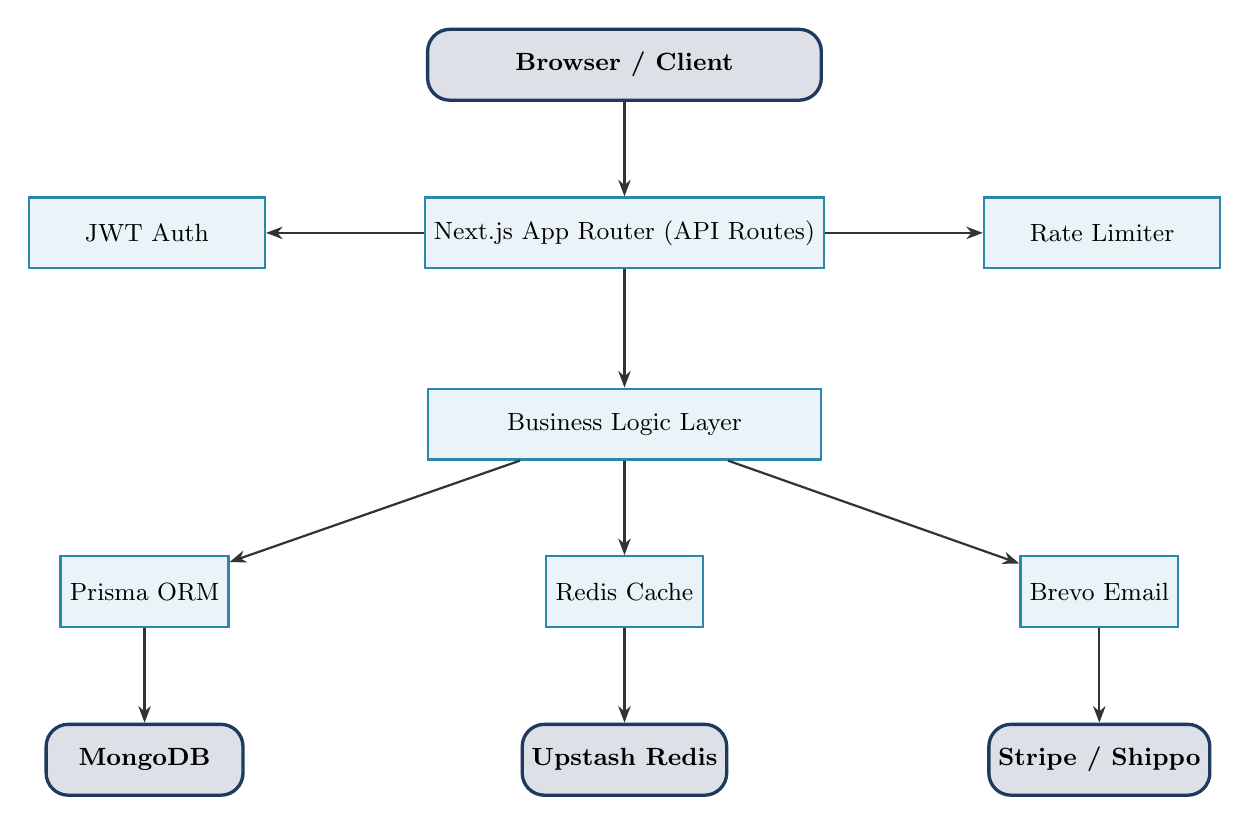
\begin{tikzpicture}[node distance=1.2cm, every node/.style={font=\small}]

  % Client Layer
  \node[startstop, minimum width=5cm] (browser) {Browser / Client};

  % API Layer
  \node[process, minimum width=5cm, below=of browser] (nextjs) {Next.js App Router (API Routes)};

  % Middleware
  \node[process, minimum width=3cm, right=2cm of nextjs] (ratelimit) {Rate Limiter};
  \node[process, minimum width=3cm, left=2cm of nextjs] (auth) {JWT Auth};

  % Business Logic
  \node[process, minimum width=5cm, below=1.5cm of nextjs] (bizlogic) {Business Logic Layer};

  % Services
  \node[process, minimum width=2cm, below left=1.2cm and 2.5cm of bizlogic] (prisma) {Prisma ORM};
  \node[process, minimum width=2cm, below=1.2cm of bizlogic] (cache) {Redis Cache};
  \node[process, minimum width=2cm, below right=1.2cm and 2.5cm of bizlogic] (email) {Brevo Email};

  % DB
  \node[startstop, minimum width=2.5cm, below=1.2cm of prisma] (mongo) {MongoDB};
  \node[startstop, minimum width=2.5cm, below=1.2cm of cache] (upstash) {Upstash Redis};
  \node[startstop, minimum width=2.5cm, below=1.2cm of email] (stripe) {Stripe / Shippo};

  % Arrows
  \draw[arrow] (browser) -- (nextjs);
  \draw[arrow] (nextjs) -- (auth);
  \draw[arrow] (nextjs) -- (ratelimit);
  \draw[arrow] (nextjs) -- (bizlogic);
  \draw[arrow] (bizlogic) -- (prisma);
  \draw[arrow] (bizlogic) -- (cache);
  \draw[arrow] (bizlogic) -- (email);
  \draw[arrow] (prisma) -- (mongo);
  \draw[arrow] (cache) -- (upstash);
  \draw[arrow] (email) -- (stripe);

\end{tikzpicture}
\caption{High-level system architecture of Stockly}
\end{figure}


% ══════════════════════════════════════════════════════════════════════════════
\chapter{Module 1: Authentication \& Session Management}
% ══════════════════════════════════════════════════════════════════════════════

\textbf{Source Files:} \texttt{utils/auth.ts}, \texttt{app/api/auth/login/route.ts}

\section{Internal Logic Walkthrough}

\subsection{verifyToken --- Branch Map}

\begin{tcolorbox}[warningbox, title={Security Critical Function}]
\texttt{verifyToken} has 5 distinct branches. All must be covered. The JWT\_SECRET
defaults to \texttt{"your\_jwt\_secret"} if the environment variable is not set ---
this is a \textbf{critical security risk} in production.
\end{tcolorbox}

\begin{center}
\begin{tabular}{clp{7cm}}
  \toprule
  \textbf{Branch} & \textbf{Condition} & \textbf{Result} \\
  \midrule
  A & \texttt{token} is falsy, \texttt{"null"}, or \texttt{"undefined"} & \texttt{return null} \\
  B & \texttt{isServer === false} (client-side execution) & \texttt{return null} \\
  C & \texttt{jwt} is undefined or \texttt{jwt.verify} missing & \texttt{return null} \\
  D & \texttt{jwt.verify} throws (expired / invalid / malformed) & \texttt{catch} $\to$ \texttt{return null} \\
  E & \texttt{jwt.verify} succeeds & \texttt{return \{ userId \}} \\
  \bottomrule
\end{tabular}
\end{center}

\subsection{verifyToken Control Flow Diagram}

\begin{figure}[h!]
\centering
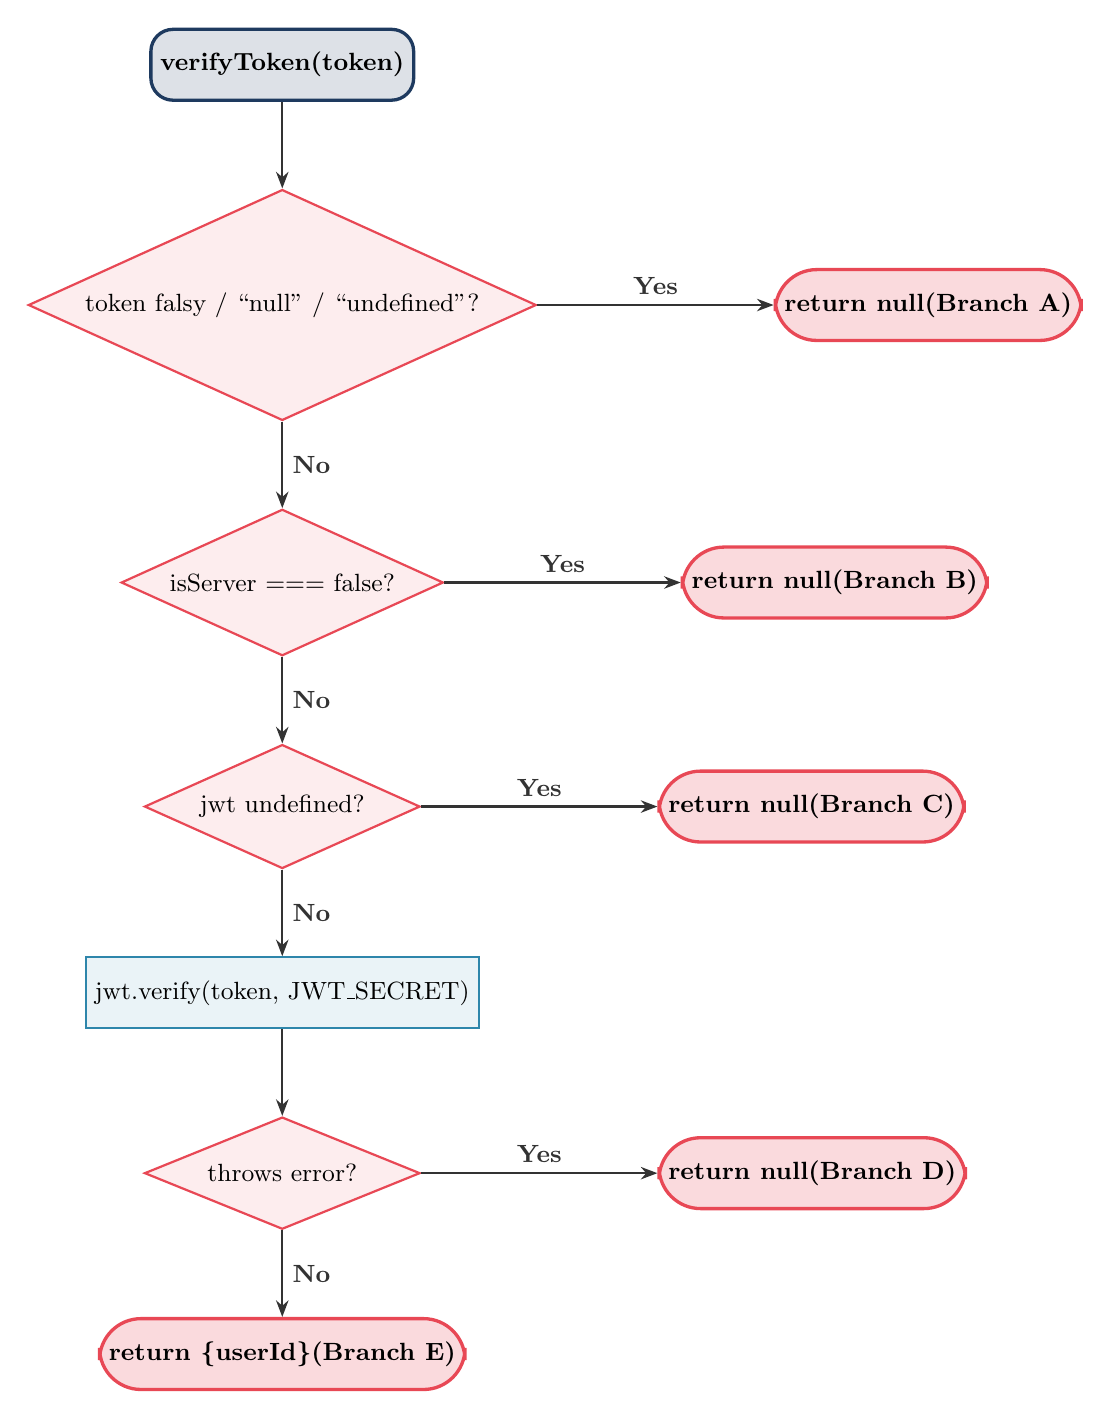
\begin{tikzpicture}[node distance=1.1cm]

  \node[startstop] (start) {verifyToken(token)};
  \node[decision, below=of start] (d1) {token falsy / ``null'' / ``undefined''?};
  \node[terminal, right=3cm of d1] (rA) {return null \\ \small(Branch A)};
  \node[decision, below=of d1] (d2) {isServer === false?};
  \node[terminal, right=3cm of d2] (rB) {return null \\ \small(Branch B)};
  \node[decision, below=of d2] (d3) {jwt undefined?};
  \node[terminal, right=3cm of d3] (rC) {return null \\ \small(Branch C)};
  \node[process, below=of d3] (verify) {jwt.verify(token, JWT\_SECRET)};
  \node[decision, below=of verify] (d4) {throws error?};
  \node[terminal, right=3cm of d4] (rD) {return null \\ \small(Branch D)};
  \node[terminal, below=of d4] (rE) {return \{userId\} \\ \small(Branch E)};

  \draw[arrow] (start) -- (d1);
  \draw[arrow] (d1) -- node[yes, above]{Yes} (rA);
  \draw[arrow] (d1) -- node[no, right]{No} (d2);
  \draw[arrow] (d2) -- node[yes, above]{Yes} (rB);
  \draw[arrow] (d2) -- node[no, right]{No} (d3);
  \draw[arrow] (d3) -- node[yes, above]{Yes} (rC);
  \draw[arrow] (d3) -- node[no, right]{No} (verify);
  \draw[arrow] (verify) -- (d4);
  \draw[arrow] (d4) -- node[yes, above]{Yes} (rD);
  \draw[arrow] (d4) -- node[no, right]{No} (rE);

\end{tikzpicture}
\caption{Control flow diagram for \texttt{verifyToken}}
\end{figure}

\subsection{Login Route Decision Tree}

\begin{figure}[h!]
\centering
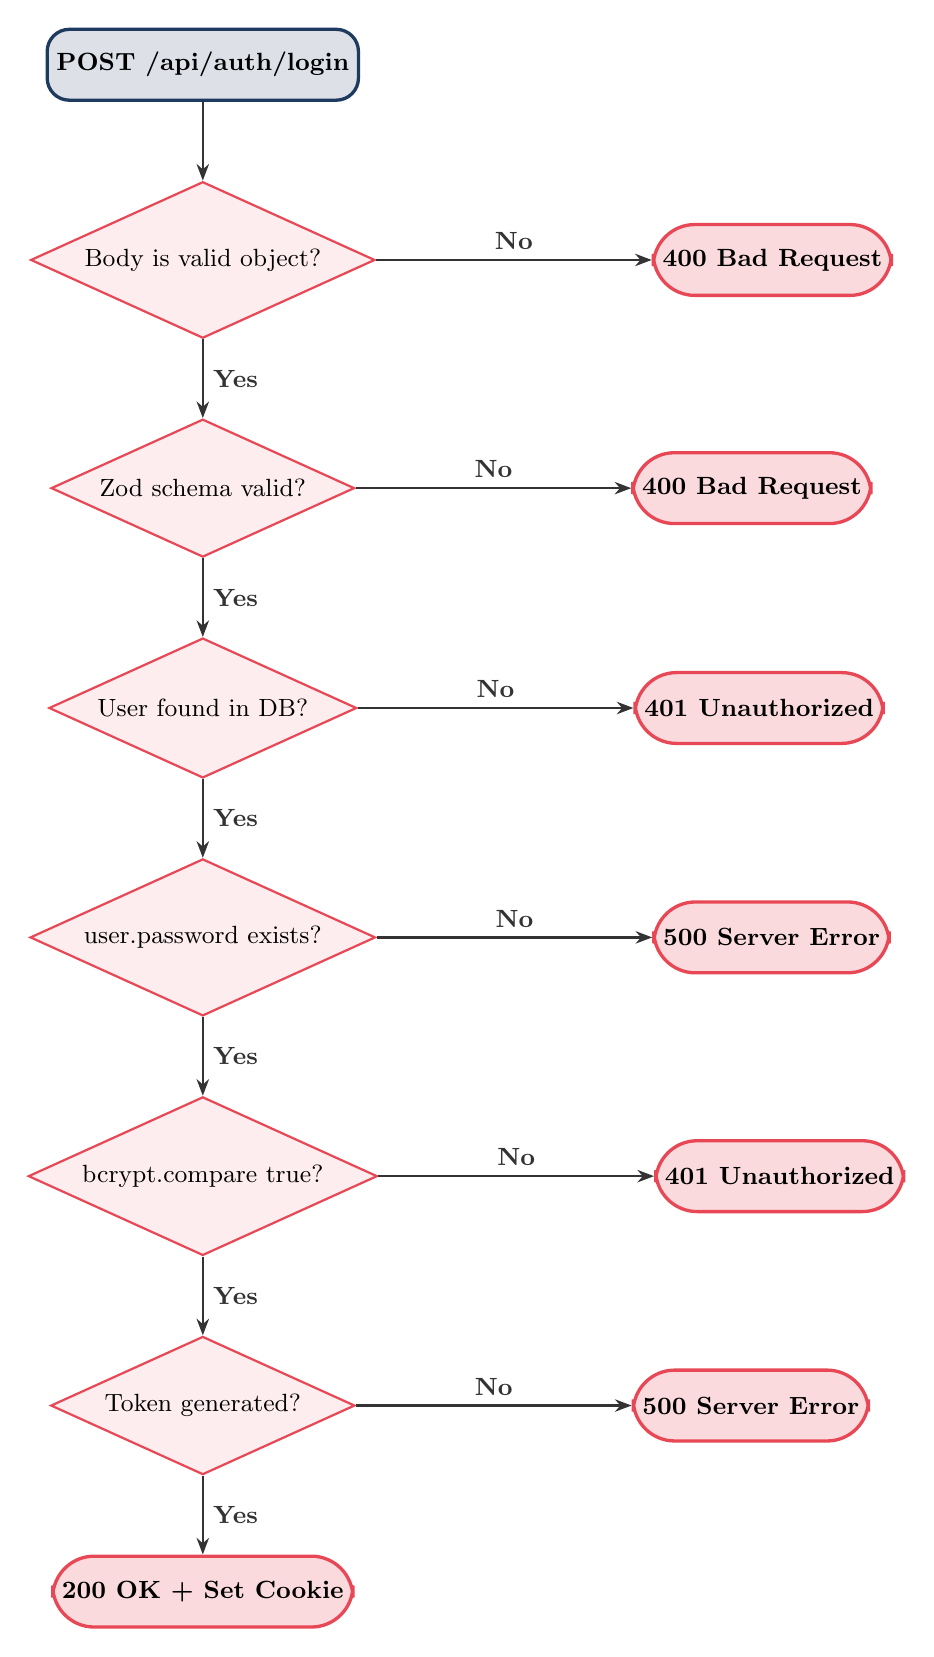
\begin{tikzpicture}[node distance=1.0cm]

  \node[startstop] (start) {POST /api/auth/login};
  \node[decision, below=of start] (d1) {Body is valid object?};
  \node[terminal, right=3.5cm of d1] (r400a) {400 Bad Request};
  \node[decision, below=of d1] (d2) {Zod schema valid?};
  \node[terminal, right=3.5cm of d2] (r400b) {400 Bad Request};
  \node[decision, below=of d2] (d3) {User found in DB?};
  \node[terminal, right=3.5cm of d3] (r401a) {401 Unauthorized};
  \node[decision, below=of d3] (d4) {user.password exists?};
  \node[terminal, right=3.5cm of d4] (r500a) {500 Server Error};
  \node[decision, below=of d4] (d5) {bcrypt.compare true?};
  \node[terminal, right=3.5cm of d5] (r401b) {401 Unauthorized};
  \node[decision, below=of d5] (d6) {Token generated?};
  \node[terminal, right=3.5cm of d6] (r500b) {500 Server Error};
  \node[terminal, below=of d6] (r200) {200 OK + Set Cookie};

  \draw[arrow] (start) -- (d1);
  \draw[arrow] (d1) -- node[no, above]{No} (r400a);
  \draw[arrow] (d1) -- node[yes, right]{Yes} (d2);
  \draw[arrow] (d2) -- node[no, above]{No} (r400b);
  \draw[arrow] (d2) -- node[yes, right]{Yes} (d3);
  \draw[arrow] (d3) -- node[no, above]{No} (r401a);
  \draw[arrow] (d3) -- node[yes, right]{Yes} (d4);
  \draw[arrow] (d4) -- node[no, above]{No} (r500a);
  \draw[arrow] (d4) -- node[yes, right]{Yes} (d5);
  \draw[arrow] (d5) -- node[no, above]{No} (r401b);
  \draw[arrow] (d5) -- node[yes, right]{Yes} (d6);
  \draw[arrow] (d6) -- node[no, above]{No} (r500b);
  \draw[arrow] (d6) -- node[yes, right]{Yes} (r200);

\end{tikzpicture}
\caption{Login route complete decision tree}
\end{figure}

\section{Test Cases --- Authentication}

\begin{tcolorbox}[testbox, title={AUTH-001 \hfill \pone}]
\textbf{Function:} \texttt{verifyToken} \\
\textbf{Scenario:} Token is an empty string \\
\textbf{Input:} \texttt{token = ""} \\
\textbf{Expected Path:} Branch A (falsy check) $\to$ \texttt{return null} \\
\textbf{Expected Output:} \texttt{null} \\
\textbf{Coverage:} Statement + Branch A
\end{tcolorbox}

\begin{tcolorbox}[testbox, title={AUTH-002 \hfill \pone}]
\textbf{Function:} \texttt{verifyToken} \\
\textbf{Scenario:} Token is the string \texttt{"null"} \\
\textbf{Input:} \texttt{token = "null"} \\
\textbf{Expected Path:} Branch A (string \texttt{"null"} check) $\to$ \texttt{return null} \\
\textbf{Expected Output:} \texttt{null} \\
\textbf{Coverage:} Branch A edge case
\end{tcolorbox}

\begin{tcolorbox}[testbox, title={AUTH-003 \hfill \pone}]
\textbf{Function:} \texttt{verifyToken} \\
\textbf{Scenario:} Token is the string \texttt{"undefined"} \\
\textbf{Input:} \texttt{token = "undefined"} \\
\textbf{Expected Path:} Branch A $\to$ \texttt{return null} \\
\textbf{Expected Output:} \texttt{null} \\
\textbf{Coverage:} Branch A edge case
\end{tcolorbox}

\begin{tcolorbox}[testbox, title={AUTH-004 \hfill \pone}]
\textbf{Function:} \texttt{verifyToken} \\
\textbf{Scenario:} Valid JWT token on server side \\
\textbf{Input:} Token generated by \texttt{generateToken("user123")} \\
\textbf{Expected Path:} Branch E $\to$ \texttt{return \{ userId: "user123" \}} \\
\textbf{Expected Output:} \texttt{\{ userId: "user123" \}} \\
\textbf{Coverage:} Happy path
\end{tcolorbox}

\begin{tcolorbox}[criticalbox, title={AUTH-005 \hfill \pone\ --- Expired Token}]
\textbf{Function:} \texttt{verifyToken} \\
\textbf{Scenario:} Expired JWT token \\
\textbf{Input:} Token with \texttt{expiresIn: "1ms"}, verified after 10ms delay \\
\textbf{Expected Path:} Branch D $\to$ \texttt{jwt.verify} throws \texttt{TokenExpiredError} $\to$ \texttt{return null} \\
\textbf{Expected Output:} \texttt{null} \\
\textbf{Coverage:} Exception handling branch
\end{tcolorbox}

\begin{tcolorbox}[criticalbox, title={AUTH-006 \hfill \pone\ --- Wrong Secret (Security)}]
\textbf{Function:} \texttt{verifyToken} \\
\textbf{Scenario:} Token signed with wrong secret \\
\textbf{Input:} \texttt{jwt.sign(\{ userId: "x" \}, "WRONG\_SECRET")} \\
\textbf{Expected Path:} Branch D $\to$ \texttt{jwt.verify} throws \texttt{JsonWebTokenError} $\to$ \texttt{return null} \\
\textbf{Expected Output:} \texttt{null} \\
\textbf{Coverage:} Security branch
\end{tcolorbox}

\begin{tcolorbox}[testbox, title={AUTH-007 \hfill \pone}]
\textbf{Function:} \texttt{verifyToken} \\
\textbf{Scenario:} Malformed / random string token \\
\textbf{Input:} \texttt{token = "not.a.jwt.token"} \\
\textbf{Expected Path:} Branch D $\to$ catch $\to$ \texttt{return null} \\
\textbf{Expected Output:} \texttt{null} \\
\textbf{Coverage:} Malformed input
\end{tcolorbox}

\begin{tcolorbox}[testbox, title={AUTH-008 \hfill \pone}]
\textbf{Function:} \texttt{generateToken} \\
\textbf{Scenario:} Valid userId generates a decodable token \\
\textbf{Input:} \texttt{userId = "abc123"} \\
\textbf{Expected:} \texttt{jwt.decode(result).userId === "abc123"} \\
\textbf{Coverage:} Token payload integrity
\end{tcolorbox}

\begin{tcolorbox}[testbox, title={AUTH-009 \hfill \pone}]
\textbf{Function:} \texttt{hashPassword} + \texttt{comparePassword} \\
\textbf{Scenario:} Hash then compare same password (round-trip) \\
\textbf{Input:} \texttt{password = "SecurePass123!"} \\
\textbf{Steps:} (1) \texttt{hash = await hashPassword(password)} \quad (2) \texttt{result = await comparePassword(password, hash)} \\
\textbf{Expected:} \texttt{result === true} \\
\textbf{Coverage:} Round-trip password verification
\end{tcolorbox}

\begin{tcolorbox}[testbox, title={AUTH-010 \hfill \pone}]
\textbf{Function:} \texttt{comparePassword} \\
\textbf{Scenario:} Wrong password against valid hash \\
\textbf{Input:} \texttt{comparePassword("WrongPass", hashOf("CorrectPass"))} \\
\textbf{Expected:} \texttt{false} \\
\textbf{Coverage:} Negative comparison branch
\end{tcolorbox}

\begin{tcolorbox}[testbox, title={AUTH-011 \hfill \pone}]
\textbf{Route:} \texttt{POST /api/auth/login} \\
\textbf{Scenario:} Missing email field in body \\
\textbf{Input:} \texttt{\{ password: "test123" \}} \\
\textbf{Expected Path:} \texttt{loginSchema.parse} throws \texttt{ZodError} $\to$ 400 \\
\textbf{Expected Response:} \texttt{\{ error: "..." \}}, status \textbf{400} \\
\textbf{Coverage:} Zod validation branch
\end{tcolorbox}

\begin{tcolorbox}[testbox, title={AUTH-012 \hfill \pone}]
\textbf{Route:} \texttt{POST /api/auth/login} \\
\textbf{Scenario:} User not found in database \\
\textbf{Input:} \texttt{\{ email: "nonexistent@test.com", password: "pass" \}} \\
\textbf{Mock:} \texttt{prisma.user.findUnique} returns \texttt{null} \\
\textbf{Expected Path:} \texttt{user === null} $\to$ 401 \\
\textbf{Expected Response:} \texttt{\{ error: "Invalid email or password" \}}, status \textbf{401} \\
\textbf{Coverage:} User not found branch
\end{tcolorbox}

\begin{tcolorbox}[criticalbox, title={AUTH-013 \hfill \ptwo\ --- Corrupted Data}]
\textbf{Route:} \texttt{POST /api/auth/login} \\
\textbf{Scenario:} User found but \texttt{password} field is \texttt{null} \\
\textbf{Mock:} \texttt{prisma.user.findUnique} returns \texttt{\{ id: "x", password: null \}} \\
\textbf{Expected Path:} \texttt{!user.password} $\to$ 500 \\
\textbf{Expected Response:} \texttt{\{ error: "User data corrupted: password missing" \}}, status \textbf{500} \\
\textbf{Coverage:} Data corruption branch
\end{tcolorbox}

\begin{tcolorbox}[testbox, title={AUTH-014 \hfill \pone}]
\textbf{Route:} \texttt{POST /api/auth/login} \\
\textbf{Scenario:} Correct credentials --- full happy path \\
\textbf{Input:} \texttt{\{ email: "admin@test.com", password: "correct" \}} \\
\textbf{Mock:} User found, \texttt{bcrypt.compare} returns \texttt{true} \\
\textbf{Expected Response:} Status \textbf{200}, \texttt{Set-Cookie} header with \texttt{session\_id} \\
\textbf{Coverage:} Full happy path
\end{tcolorbox}

\begin{tcolorbox}[testbox, title={AUTH-015 \hfill \pone}]
\textbf{Function:} \texttt{getSessionFromRequest} \\
\textbf{Scenario:} No \texttt{session\_id} cookie present \\
\textbf{Input:} Request with no cookies \\
\textbf{Expected Path:} \texttt{cookie === undefined} $\to$ \texttt{return null} \\
\textbf{Expected Output:} \texttt{null} \\
\textbf{Coverage:} Missing cookie branch
\end{tcolorbox}

\begin{tcolorbox}[testbox, title={AUTH-016 \hfill \ptwo}]
\textbf{Function:} \texttt{getSessionFromRequest} \\
\textbf{Scenario:} Valid cookie but user deleted from DB \\
\textbf{Mock:} \texttt{prisma.user.findUnique} returns \texttt{null} \\
\textbf{Expected Path:} Decoded OK $\to$ DB query $\to$ \texttt{null} \\
\textbf{Expected Output:} \texttt{null} \\
\textbf{Coverage:} Deleted user edge case
\end{tcolorbox}


% ══════════════════════════════════════════════════════════════════════════════
\chapter{Module 2: Order Management \& Stock State Machine}
% ══════════════════════════════════════════════════════════════════════════════

\textbf{Source Files:} \texttt{prisma/order.ts}, \texttt{app/api/orders/route.ts}

\section{Stock Reservation State Machine}

\begin{tcolorbox}[criticalbox, title={Critical Business Logic --- Stock Reservation}]
\begin{itemize}
  \item \textbf{Order CREATE (pending):} \texttt{reservedQuantity} \textbf{INCREASES} (stock reserved, not deducted)
  \item \textbf{Order CONFIRM / PAY:} \texttt{quantity} \textbf{DECREASES}, \texttt{reservedQuantity} \textbf{DECREASES}
  \item \textbf{Order CANCEL (was pending):} \texttt{reservedQuantity} \textbf{DECREASES} (reservation released)
  \item \textbf{Order CANCEL (was confirmed/paid):} \texttt{quantity} \textbf{INCREASES} (stock restored)
  \item \textbf{Available Stock Formula:} $\text{availableStock} = \text{quantity} - \text{reservedQuantity}$
\end{itemize}
\end{tcolorbox}

\subsection{Order Status State Machine Diagram}

\begin{figure}[h!]
\centering
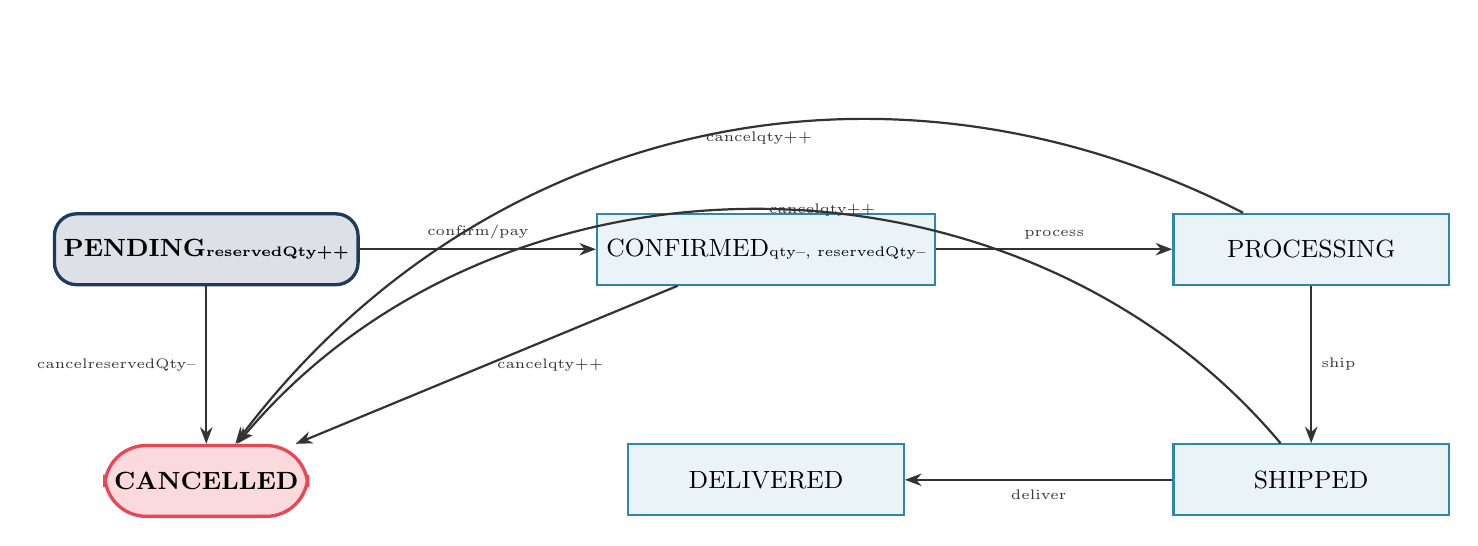
\begin{tikzpicture}[node distance=1.8cm, every node/.style={font=\small}]

  \node[startstop] (pending) {PENDING \\ \tiny reservedQty++};
  \node[process, right=3cm of pending] (confirmed) {CONFIRMED \\ \tiny qty--, reservedQty--};
  \node[process, right=3cm of confirmed] (processing) {PROCESSING};
  \node[process, below=2cm of processing] (shipped) {SHIPPED};
  \node[process, below=2cm of confirmed] (delivered) {DELIVERED};
  \node[terminal, below=2cm of pending] (cancelled) {CANCELLED};

  \draw[arrow] (pending) -- node[above]{\tiny confirm/pay} (confirmed);
  \draw[arrow] (confirmed) -- node[above]{\tiny process} (processing);
  \draw[arrow] (processing) -- node[right]{\tiny ship} (shipped);
  \draw[arrow] (shipped) -- node[below]{\tiny deliver} (delivered);
  \draw[arrow] (pending) -- node[left]{\tiny cancel \\ \tiny reservedQty--} (cancelled);
  \draw[arrow] (confirmed) -- node[right]{\tiny cancel \\ \tiny qty++} (cancelled);
  \draw[arrow] (processing) to[bend right=40] node[right]{\tiny cancel \\ \tiny qty++} (cancelled);
  \draw[arrow] (shipped) to[bend right=50] node[right]{\tiny cancel \\ \tiny qty++} (cancelled);

\end{tikzpicture}
\caption{Order status state machine with stock side-effects}
\end{figure}

\subsection{createOrder Control Flow Diagram}

\begin{figure}[h!]
\centering
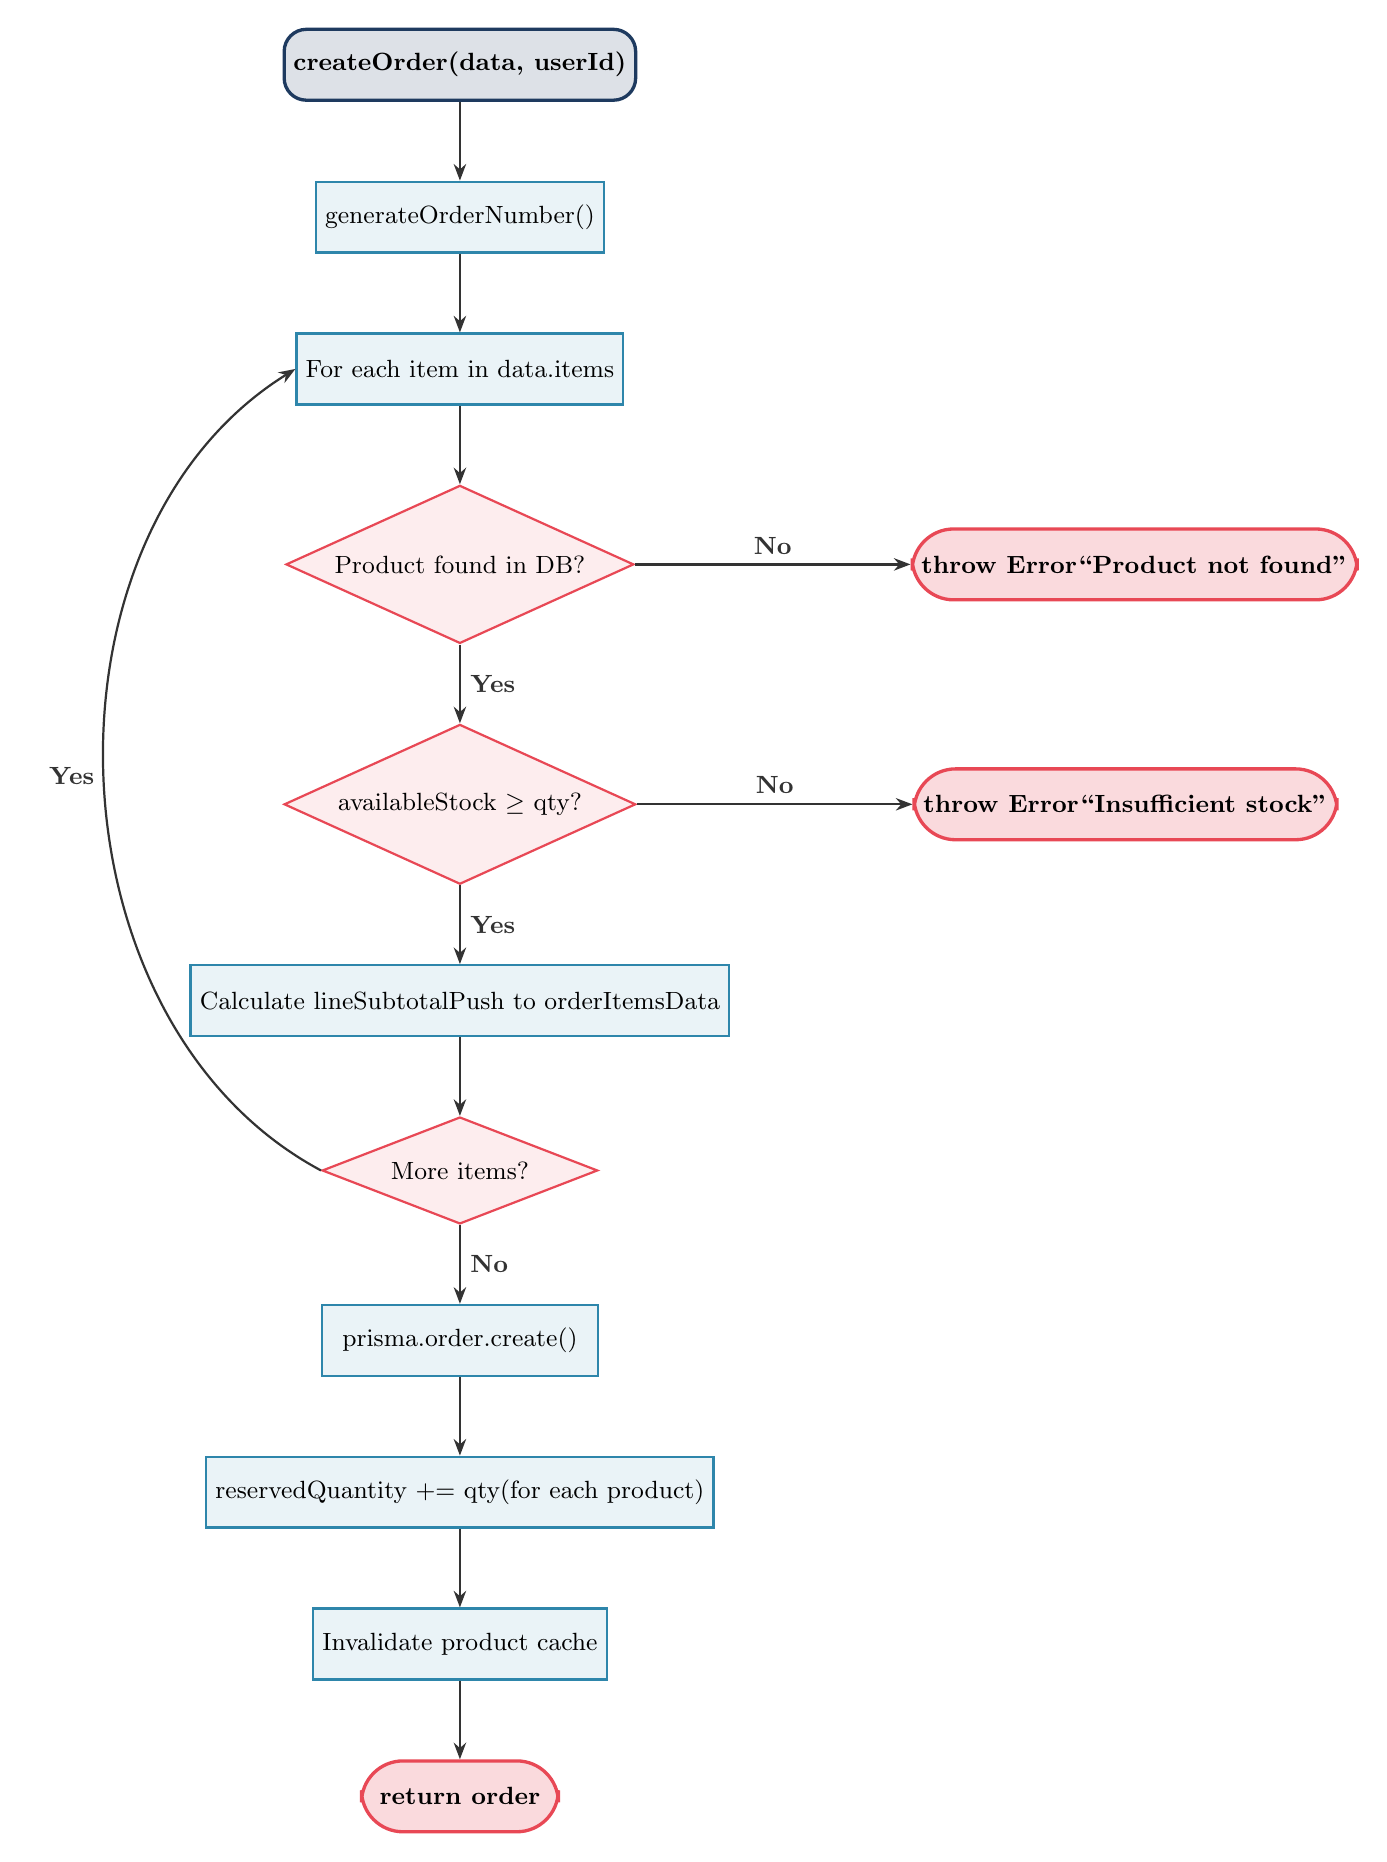
\begin{tikzpicture}[node distance=1.0cm]

  \node[startstop] (start) {createOrder(data, userId)};
  \node[process, below=of start] (gennum) {generateOrderNumber()};
  \node[process, below=of gennum] (loop) {For each item in data.items};
  \node[decision, below=of loop] (d1) {Product found in DB?};
  \node[terminal, right=3.5cm of d1] (err1) {throw Error \\ ``Product not found''};
  \node[decision, below=of d1] (d2) {availableStock $\geq$ qty?};
  \node[terminal, right=3.5cm of d2] (err2) {throw Error \\ ``Insufficient stock''};
  \node[process, below=of d2] (calc) {Calculate lineSubtotal \\ Push to orderItemsData};
  \node[decision, below=of calc] (d3) {More items?};
  \node[process, below=of d3] (create) {prisma.order.create()};
  \node[process, below=of create] (reserve) {reservedQuantity += qty \\ (for each product)};
  \node[process, below=of reserve] (cache) {Invalidate product cache};
  \node[terminal, below=of cache] (ret) {return order};

  \draw[arrow] (start) -- (gennum);
  \draw[arrow] (gennum) -- (loop);
  \draw[arrow] (loop) -- (d1);
  \draw[arrow] (d1) -- node[no, above]{No} (err1);
  \draw[arrow] (d1) -- node[yes, right]{Yes} (d2);
  \draw[arrow] (d2) -- node[no, above]{No} (err2);
  \draw[arrow] (d2) -- node[yes, right]{Yes} (calc);
  \draw[arrow] (calc) -- (d3);
  \draw[arrow] (d3.west) to[bend left=60] node[yes, left]{Yes} (loop.west);
  \draw[arrow] (d3) -- node[no, right]{No} (create);
  \draw[arrow] (create) -- (reserve);
  \draw[arrow] (reserve) -- (cache);
  \draw[arrow] (cache) -- (ret);

\end{tikzpicture}
\caption{createOrder complete control flow}
\end{figure}

\section{Test Cases --- Order Management}

\begin{tcolorbox}[testbox, title={ORD-001 \hfill \ptwo}]
\textbf{Function:} \texttt{generateOrderNumber} \\
\textbf{Scenario:} First order of the day (0 existing orders today) \\
\textbf{Mock:} \texttt{prisma.order.count} returns \texttt{0} \\
\textbf{Expected:} Sequence part = \texttt{"0001"}, format: \texttt{ORD-2026-0401-HHMMSS-0001} \\
\textbf{Coverage:} Sequence generation, zero-count branch
\end{tcolorbox}

\begin{tcolorbox}[testbox, title={ORD-002 \hfill \pthree\ --- Boundary}]
\textbf{Function:} \texttt{generateOrderNumber} \\
\textbf{Scenario:} 9999 orders already exist today \\
\textbf{Mock:} \texttt{prisma.order.count} returns \texttt{9999} \\
\textbf{Expected:} Sequence = \texttt{"10000"} (5 digits, overflow of 4-digit pad) \\
\textbf{Note:} Race condition possible under high concurrency --- not atomic \\
\textbf{Coverage:} Boundary value, sequence overflow
\end{tcolorbox}

\begin{tcolorbox}[criticalbox, title={ORD-003 \hfill \pone\ --- Product Not Found}]
\textbf{Function:} \texttt{createOrder} \\
\textbf{Scenario:} Product not found in database \\
\textbf{Input:} \texttt{data.items = [\{ productId: "nonexistent", quantity: 1 \}]} \\
\textbf{Mock:} \texttt{prisma.product.findUnique} returns \texttt{null} \\
\textbf{Expected:} \texttt{throw Error("Product not found: nonexistent")} \\
\textbf{Coverage:} Product not found branch
\end{tcolorbox}

\begin{tcolorbox}[criticalbox, title={ORD-004 \hfill \pone\ --- Insufficient Stock}]
\textbf{Function:} \texttt{createOrder} \\
\textbf{Scenario:} Insufficient available stock \\
\textbf{Input:} \texttt{item.quantity = 10} \\
\textbf{Mock:} \texttt{product.quantity = 15}, \texttt{product.reservedQuantity = 8} \\
\textbf{Internal:} $\text{availableStock} = 15 - 8 = 7 < 10$ \\
\textbf{Expected:} \texttt{throw Error("Insufficient stock. Available: 7, Requested: 10")} \\
\textbf{Coverage:} Stock check branch (insufficient)
\end{tcolorbox}

\begin{tcolorbox}[testbox, title={ORD-005 \hfill \pone\ --- Exact Stock Boundary}]
\textbf{Function:} \texttt{createOrder} \\
\textbf{Scenario:} Exactly enough stock (boundary value) \\
\textbf{Input:} \texttt{item.quantity = 7} \\
\textbf{Mock:} \texttt{product.quantity = 15}, \texttt{product.reservedQuantity = 8} \\
\textbf{Internal:} $\text{availableStock} = 7 = 7$ (exactly enough) \\
\textbf{Expected:} Order created successfully, no error \\
\textbf{Coverage:} Boundary value (exact stock match)
\end{tcolorbox}

\begin{tcolorbox}[criticalbox, title={ORD-006 \hfill \pone\ --- Boundary + 1}]
\textbf{Function:} \texttt{createOrder} \\
\textbf{Scenario:} One more than available stock \\
\textbf{Input:} \texttt{item.quantity = 8} \\
\textbf{Mock:} \texttt{product.quantity = 15}, \texttt{product.reservedQuantity = 8} \\
\textbf{Internal:} $\text{availableStock} = 7 < 8$ \\
\textbf{Expected:} \texttt{throw Error("Insufficient stock")} \\
\textbf{Coverage:} Boundary value + 1
\end{tcolorbox}

\begin{tcolorbox}[testbox, title={ORD-007 \hfill \ptwo}]
\textbf{Function:} \texttt{createOrder} \\
\textbf{Scenario:} \texttt{reservedQuantity} is \texttt{null} (not yet set) \\
\textbf{Mock:} \texttt{product.quantity = 10}, \texttt{product.reservedQuantity = null} \\
\textbf{Internal:} $\text{availableStock} = 10 - \texttt{Number(null)} = 10 - 0 = 10$ \\
\textbf{Expected:} \texttt{availableStock} correctly computed as \texttt{10} \\
\textbf{Coverage:} Null coalescing in stock calculation
\end{tcolorbox}

\begin{tcolorbox}[criticalbox, title={ORD-008 \hfill \pone\ --- Atomicity Gap}]
\textbf{Function:} \texttt{createOrder} \\
\textbf{Scenario:} Multiple items, second item fails stock check \\
\textbf{Input:} \texttt{items = [\{ productA, qty: 1 \}, \{ productB, qty: 999 \}]} \\
\textbf{Mock:} productA has stock, productB has only 5 \\
\textbf{Expected:} Error thrown on productB; \textbf{NO} reservation made for productA \\
\textbf{Note:} Tests fail-fast behaviour before any DB writes \\
\textbf{Coverage:} Partial failure rollback (atomicity check)
\end{tcolorbox}

\begin{tcolorbox}[testbox, title={ORD-009 \hfill \pone}]
\textbf{Function:} \texttt{createOrder} \\
\textbf{Scenario:} Tax, shipping, discount all provided \\
\textbf{Input:} \texttt{subtotal=100, tax=10, shipping=5, discount=15} \\
\textbf{Expected:} $\text{total} = 100 + 10 + 5 - 15 = 100$ \\
\textbf{Coverage:} Total calculation formula
\end{tcolorbox}

\begin{tcolorbox}[testbox, title={ORD-010 \hfill \ptwo}]
\textbf{Function:} \texttt{createOrder} \\
\textbf{Scenario:} Tax and shipping are 0 (falsy) \\
\textbf{Input:} \texttt{tax=0, shipping=0, discount=0} \\
\textbf{Internal:} \texttt{tax > 0} is \texttt{false} $\to$ stored as \texttt{null} \\
\textbf{Expected:} \texttt{order.tax = null}, \texttt{order.shipping = null}, \texttt{order.discount = null} \\
\textbf{Coverage:} Falsy-to-null conversion branches
\end{tcolorbox}

\begin{tcolorbox}[testbox, title={ORD-011 \hfill \pone}]
\textbf{Function:} \texttt{createOrder} \\
\textbf{Scenario:} Verify \texttt{reservedQuantity} incremented after order creation \\
\textbf{Input:} Single item, \texttt{quantity = 3} \\
\textbf{Mock:} \texttt{product.reservedQuantity = 5} before order \\
\textbf{Expected:} After \texttt{createOrder}, \texttt{product.reservedQuantity = 8} \\
\textbf{Coverage:} Stock reservation side effect
\end{tcolorbox}

\begin{tcolorbox}[testbox, title={ORD-012 \hfill \pone}]
\textbf{Route:} \texttt{GET /api/orders} \\
\textbf{Scenario:} Unauthenticated request (no session cookie) \\
\textbf{Mock:} \texttt{getSessionFromRequest} returns \texttt{null} \\
\textbf{Expected:} \texttt{\{ error: "Unauthorized" \}}, status \textbf{401} \\
\textbf{Coverage:} Auth guard branch
\end{tcolorbox}

\begin{tcolorbox}[testbox, title={ORD-013 \hfill \ptwo}]
\textbf{Route:} \texttt{GET /api/orders} \\
\textbf{Scenario:} Supplier role with no supplier record \\
\textbf{Mock:} \texttt{session.role = "supplier"}, \texttt{getSupplierByUserId} returns \texttt{null} \\
\textbf{Expected:} \texttt{NextResponse.json([])} --- empty array, not error \\
\textbf{Coverage:} Supplier without record branch
\end{tcolorbox}

\begin{tcolorbox}[testbox, title={ORD-014 \hfill \ptwo}]
\textbf{Route:} \texttt{GET /api/orders} \\
\textbf{Scenario:} Cache hit for orders list \\
\textbf{Mock:} \texttt{getCache} returns cached array \\
\textbf{Expected:} Returns cached data without DB query \\
\textbf{Coverage:} Cache hit branch
\end{tcolorbox}

\begin{tcolorbox}[testbox, title={ORD-015 \hfill \pone}]
\textbf{Route:} \texttt{GET /api/orders} \\
\textbf{Scenario:} Client role fetches only their orders \\
\textbf{Mock:} \texttt{session.role = "client"}, \texttt{session.id = "clientUserId"} \\
\textbf{Expected:} \texttt{getOrdersByClientId} called with \texttt{"clientUserId"} \\
\textbf{Coverage:} Role-based query branching (client)
\end{tcolorbox}

\begin{tcolorbox}[testbox, title={ORD-016 \hfill \ptwo}]
\textbf{Route:} \texttt{GET /api/orders} \\
\textbf{Scenario:} Rate limit exceeded \\
\textbf{Mock:} \texttt{withRateLimit} returns a 429 response \\
\textbf{Expected:} 429 response returned immediately, no DB query \\
\textbf{Coverage:} Rate limit early return branch
\end{tcolorbox}


% ══════════════════════════════════════════════════════════════════════════════
\chapter{Module 3: Invoice Generation \& Financial Logic}
% ══════════════════════════════════════════════════════════════════════════════

\textbf{Source Files:} \texttt{prisma/invoice.ts}, \texttt{app/api/invoices/route.ts}

\section{Internal Logic Walkthrough}

\subsection{createInvoice Control Flow Diagram}

\begin{figure}[h!]
\centering
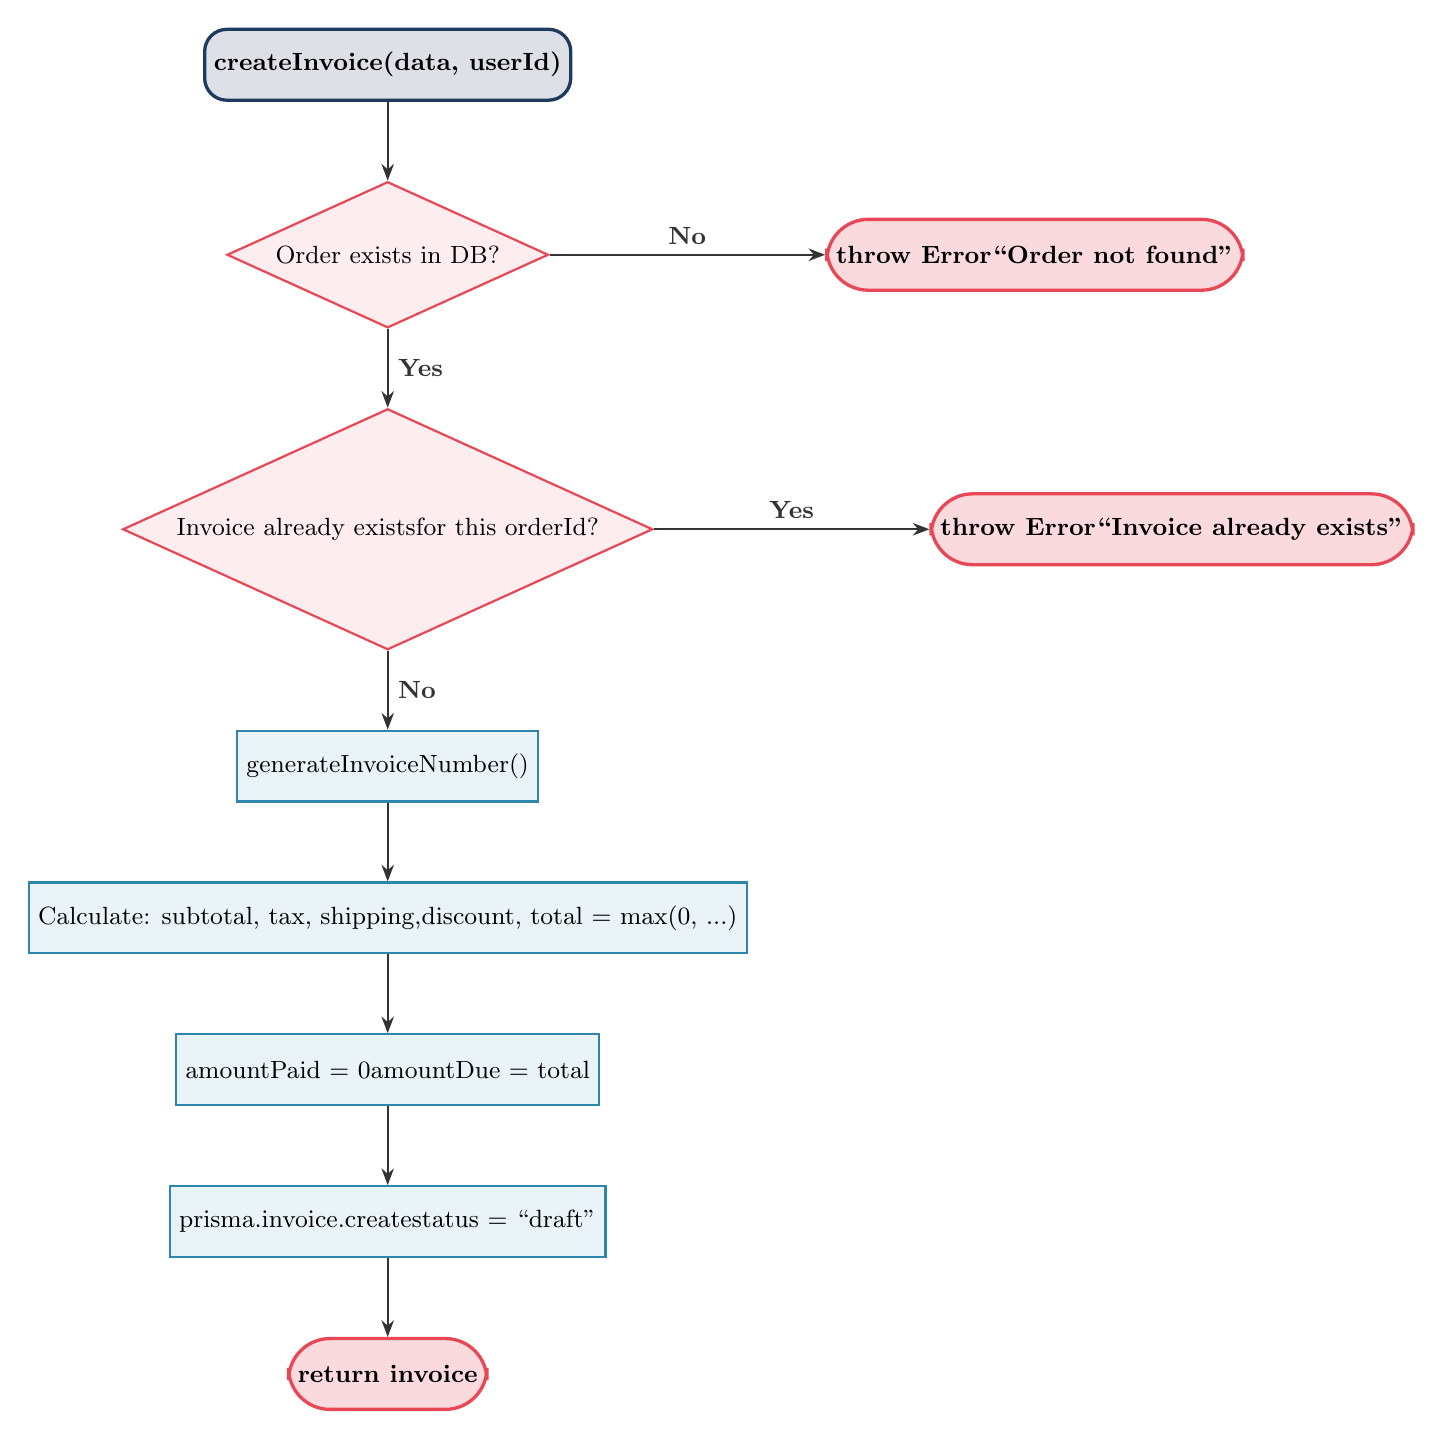
\begin{tikzpicture}[node distance=1.0cm]

  \node[startstop] (start) {createInvoice(data, userId)};
  \node[decision, below=of start] (d1) {Order exists in DB?};
  \node[terminal, right=3.5cm of d1] (err1) {throw Error \\ ``Order not found''};
  \node[decision, below=of d1] (d2) {Invoice already exists \\ for this orderId?};
  \node[terminal, right=3.5cm of d2] (err2) {throw Error \\ ``Invoice already exists''};
  \node[process, below=of d2] (gennum) {generateInvoiceNumber()};
  \node[process, below=of gennum] (calc) {Calculate: subtotal, tax, shipping, \\ discount, total = max(0, ...)};
  \node[process, below=of calc] (amounts) {amountPaid = 0 \\ amountDue = total};
  \node[process, below=of amounts] (create) {prisma.invoice.create \\ status = ``draft''};
  \node[terminal, below=of create] (ret) {return invoice};

  \draw[arrow] (start) -- (d1);
  \draw[arrow] (d1) -- node[no, above]{No} (err1);
  \draw[arrow] (d1) -- node[yes, right]{Yes} (d2);
  \draw[arrow] (d2) -- node[yes, above]{Yes} (err2);
  \draw[arrow] (d2) -- node[no, right]{No} (gennum);
  \draw[arrow] (gennum) -- (calc);
  \draw[arrow] (calc) -- (amounts);
  \draw[arrow] (amounts) -- (create);
  \draw[arrow] (create) -- (ret);

\end{tikzpicture}
\caption{createInvoice complete control flow}
\end{figure}

\subsection{generateInvoiceNumber Uniqueness Loop}

\begin{figure}[h!]
\centering
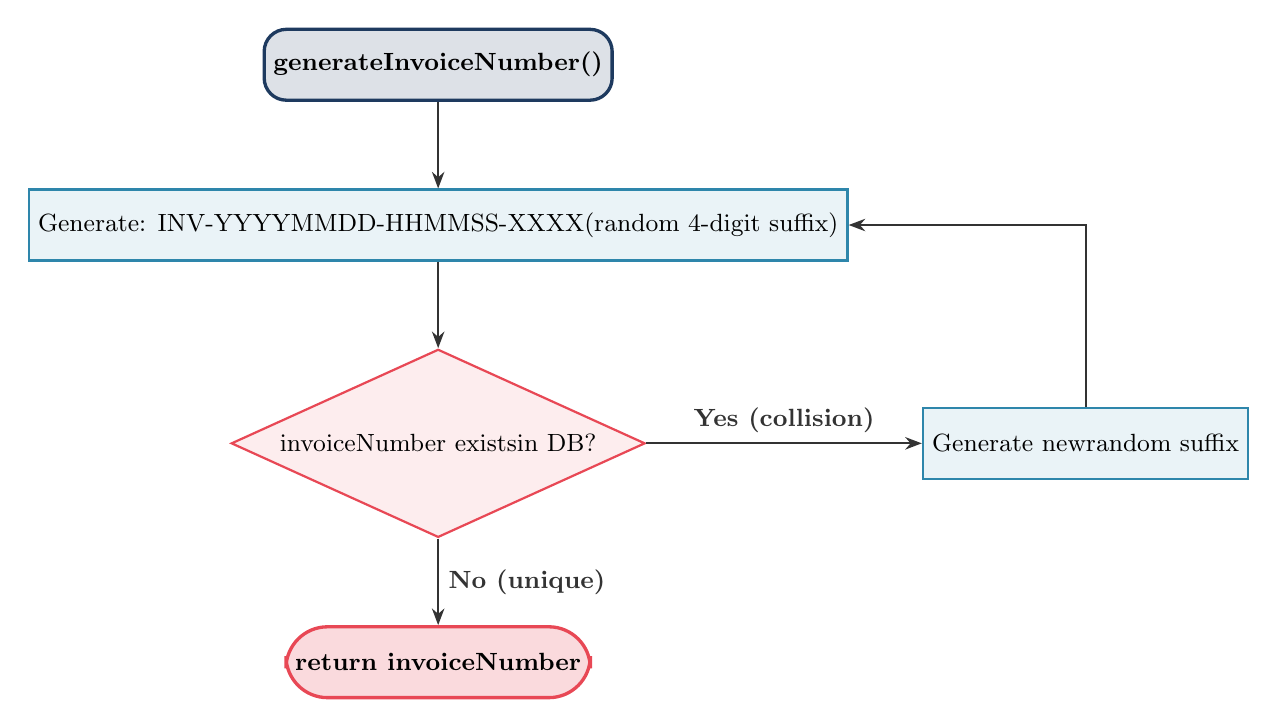
\begin{tikzpicture}[node distance=1.1cm]

  \node[startstop] (start) {generateInvoiceNumber()};
  \node[process, below=of start] (gen) {Generate: INV-YYYYMMDD-HHMMSS-XXXX \\ (random 4-digit suffix)};
  \node[decision, below=of gen] (d1) {invoiceNumber exists \\ in DB?};
  \node[process, right=3.5cm of d1] (regen) {Generate new \\ random suffix};
  \node[terminal, below=of d1] (ret) {return invoiceNumber};

  \draw[arrow] (start) -- (gen);
  \draw[arrow] (gen) -- (d1);
  \draw[arrow] (d1) -- node[yes, above]{Yes (collision)} (regen);
  \draw[arrow] (regen) |- (gen);
  \draw[arrow] (d1) -- node[no, right]{No (unique)} (ret);

\end{tikzpicture}
\caption{Invoice number uniqueness loop (collision probability = 1/9000)}
\end{figure}

\subsection{Nullish Coalescing Chain for Tax/Shipping/Discount}

\begin{tcolorbox}[infobox, title={Critical: \texttt{??} vs \texttt{||} Operator}]
The invoice uses \textbf{nullish coalescing} (\texttt{??}) not logical OR (\texttt{||}).
This means an explicit \texttt{0} from \texttt{data.tax} is \textbf{respected} and does NOT
fall back to \texttt{order.tax}. Only \texttt{null} or \texttt{undefined} trigger the fallback.

\medskip
\texttt{tax = data.tax ?? order.tax ?? 0}

\begin{center}
\begin{tabular}{lll}
  \toprule
  \texttt{data.tax} & \texttt{order.tax} & \textbf{Result} \\
  \midrule
  \texttt{20}        & \texttt{15}        & \texttt{20} (data wins) \\
  \texttt{0}         & \texttt{15}        & \texttt{0}  (explicit zero respected) \\
  \texttt{undefined} & \texttt{15}        & \texttt{15} (fallback to order) \\
  \texttt{null}      & \texttt{15}        & \texttt{15} (fallback to order) \\
  \texttt{null}      & \texttt{null}      & \texttt{0}  (final fallback) \\
  \bottomrule
\end{tabular}
\end{center}
\end{tcolorbox}

\section{Test Cases --- Invoice Generation}

\begin{tcolorbox}[testbox, title={INV-001 \hfill \ptwo}]
\textbf{Function:} \texttt{generateInvoiceNumber} \\
\textbf{Scenario:} No collision (first attempt is unique) \\
\textbf{Mock:} \texttt{prisma.invoice.findUnique} returns \texttt{null} on first call \\
\textbf{Expected:} Returns \texttt{INV-YYYYMMDD-HHMMSS-XXXX} format; while loop executes once \\
\textbf{Coverage:} Happy path, no collision
\end{tcolorbox}

\begin{tcolorbox}[testbox, title={INV-002 \hfill \ptwo}]
\textbf{Function:} \texttt{generateInvoiceNumber} \\
\textbf{Scenario:} First attempt collides, second is unique \\
\textbf{Mock:} \texttt{findUnique} returns existing invoice on call 1, \texttt{null} on call 2 \\
\textbf{Expected:} While loop executes twice, returns second generated number \\
\textbf{Coverage:} Collision handling branch (while loop iteration)
\end{tcolorbox}

\begin{tcolorbox}[testbox, title={INV-003 \hfill \ptwo}]
\textbf{Function:} \texttt{generateInvoiceNumber} \\
\textbf{Scenario:} Verify format structure \\
\textbf{Expected:} Result matches regex \texttt{/\^{}INV-\textbackslash d\{8\}-\textbackslash d\{6\}-\textbackslash d\{4\}\$/} \\
\textbf{Coverage:} Output format validation
\end{tcolorbox}

\begin{tcolorbox}[criticalbox, title={INV-004 \hfill \pone\ --- Order Not Found}]
\textbf{Function:} \texttt{createInvoice} \\
\textbf{Scenario:} Order not found \\
\textbf{Input:} \texttt{data.orderId = "nonexistent"} \\
\textbf{Mock:} \texttt{prisma.order.findUnique} returns \texttt{null} \\
\textbf{Expected:} \texttt{throw Error("Order with ID nonexistent not found")} \\
\textbf{Coverage:} Order not found branch
\end{tcolorbox}

\begin{tcolorbox}[criticalbox, title={INV-005 \hfill \pone\ --- Duplicate Invoice}]
\textbf{Function:} \texttt{createInvoice} \\
\textbf{Scenario:} Invoice already exists for this order \\
\textbf{Mock:} \texttt{prisma.invoice.findUnique} returns existing invoice \\
\textbf{Expected:} \texttt{throw Error("Invoice already exists for order \{orderId\}")} \\
\textbf{Coverage:} Duplicate invoice prevention branch
\end{tcolorbox}

\begin{tcolorbox}[testbox, title={INV-006 \hfill \pone}]
\textbf{Function:} \texttt{createInvoice} \\
\textbf{Scenario:} Total calculation with all fields \\
\textbf{Input:} \texttt{subtotal=200, tax=20, shipping=10, discount=30} \\
\textbf{Expected:} $\text{total} = \max(0,\; 200 + 20 + 10 - 30) = 200$ \\
\textbf{Coverage:} Total formula
\end{tcolorbox}

\begin{tcolorbox}[criticalbox, title={INV-007 \hfill \pone\ --- Negative Total Prevention}]
\textbf{Function:} \texttt{createInvoice} \\
\textbf{Scenario:} Discount exceeds subtotal + tax + shipping \\
\textbf{Input:} \texttt{subtotal=50, tax=5, shipping=5, discount=100} \\
\textbf{Expected:} $\text{total} = \max(0,\; 50 + 5 + 5 - 100) = \max(0, -40) = 0$ \\
\textbf{Coverage:} \texttt{Math.max(0, ...)} negative prevention branch
\end{tcolorbox}

\begin{tcolorbox}[testbox, title={INV-008 \hfill \ptwo}]
\textbf{Function:} \texttt{createInvoice} \\
\textbf{Scenario:} \texttt{data.tax} is \texttt{0} (explicit zero, not null) \\
\textbf{Input:} \texttt{data.tax = 0}, \texttt{order.tax = 15} \\
\textbf{Internal:} \texttt{tax = 0 ?? 15 = 0} \\
\textbf{Expected:} \texttt{tax = 0} (data value respected, not overridden by \texttt{order.tax}) \\
\textbf{Coverage:} Nullish coalescing vs OR operator distinction
\end{tcolorbox}

\begin{tcolorbox}[testbox, title={INV-009 \hfill \ptwo}]
\textbf{Function:} \texttt{createInvoice} \\
\textbf{Scenario:} \texttt{data.tax} is \texttt{undefined}, \texttt{order.tax} is \texttt{15} \\
\textbf{Internal:} \texttt{tax = undefined ?? 15 ?? 0 = 15} \\
\textbf{Expected:} \texttt{tax = 15} (falls back to \texttt{order.tax}) \\
\textbf{Coverage:} Fallback chain in nullish coalescing
\end{tcolorbox}

\begin{tcolorbox}[testbox, title={INV-010 \hfill \ptwo}]
\textbf{Function:} \texttt{createInvoice} \\
\textbf{Scenario:} Both \texttt{data.tax} and \texttt{order.tax} are \texttt{null} \\
\textbf{Internal:} \texttt{tax = null ?? null ?? 0 = 0} \\
\textbf{Expected:} \texttt{tax = 0} (final fallback) \\
\textbf{Coverage:} Double null fallback
\end{tcolorbox}

\begin{tcolorbox}[testbox, title={INV-011 \hfill \pone}]
\textbf{Function:} \texttt{createInvoice} \\
\textbf{Scenario:} \texttt{amountPaid} always starts at 0 \\
\textbf{Expected:} \texttt{invoice.amountPaid = 0} regardless of input; \texttt{invoice.amountDue = invoice.total} \\
\textbf{Coverage:} Initial payment state
\end{tcolorbox}

\begin{tcolorbox}[testbox, title={INV-012 \hfill \pone}]
\textbf{Function:} \texttt{createInvoice} \\
\textbf{Scenario:} Invoice status always starts as \texttt{"draft"} \\
\textbf{Expected:} \texttt{invoice.status = "draft"} \\
\textbf{Coverage:} Default status branch
\end{tcolorbox}


% ══════════════════════════════════════════════════════════════════════════════
\chapter{Module 4: Demand Forecasting Engine}
% ══════════════════════════════════════════════════════════════════════════════

\textbf{Source File:} \texttt{lib/forecasting/demand-forecast.ts}

\section{Configuration Constants}

\begin{center}
\begin{tabular}{lrl}
  \toprule
  \textbf{Constant} & \textbf{Value} & \textbf{Purpose} \\
  \midrule
  \texttt{ANALYSIS\_DAYS}     & 30  & Days of historical data to analyse \\
  \texttt{FORECAST\_DAYS}     & 14  & Days to forecast ahead \\
  \texttt{ANOMALY\_THRESHOLD} & 2.0 & Standard deviations for anomaly detection \\
  \texttt{REORDER\_LEAD\_DAYS}& 7   & Days lead time for reorder \\
  \bottomrule
\end{tabular}
\end{center}

\section{Mathematical Formulas}

\subsection{Standard Deviation (Population)}
\[
  \sigma = \sqrt{\frac{1}{N}\sum_{i=1}^{N}(x_i - \bar{x})^2}
\]

\subsection{Linear Regression Slope}
\[
  \text{slope} = \frac{n \sum x_i y_i - \sum x_i \sum y_i}{n \sum x_i^2 - (\sum x_i)^2}
\]

\subsection{Percentage Change (Trend)}
\[
  \text{percentageChange} = \frac{\text{slope} \times n \times 100}{\bar{y}} \quad (\text{if } \bar{y} > 0)
\]

\subsection{Days Until Stockout}
\[
  \text{daysUntilStockout} = \left\lfloor \frac{\text{availableStock}}{\text{predictedDailySales}} \right\rfloor \quad (\text{if predictedDailySales} > 0)
\]

\subsection{Weighted Predicted Daily Sales}
\[
  \text{predicted} = 0.7 \times \text{recentAvg} + 0.3 \times \text{overallAvg} \quad (\text{if recentDays} \geq 7)
\]

\section{analyzeTrend Control Flow Diagram}

\begin{figure}[h!]
\centering
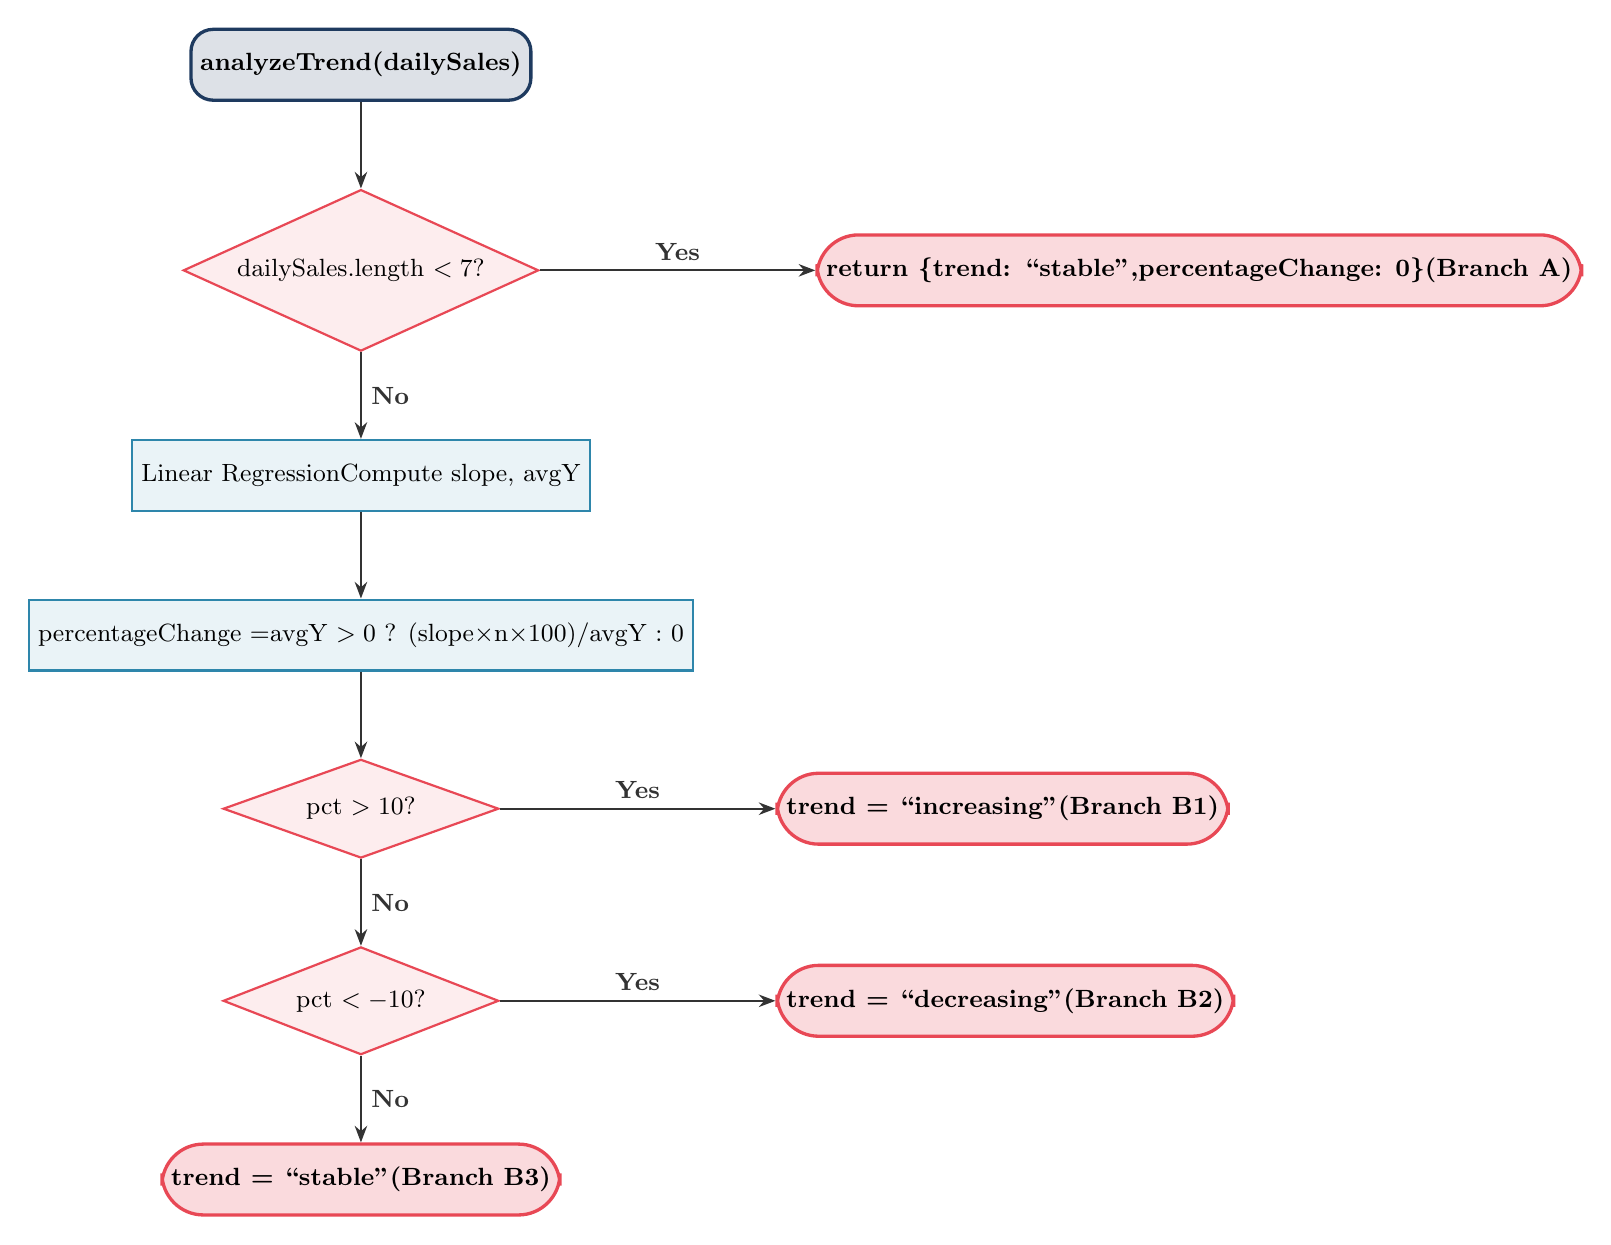
\begin{tikzpicture}[node distance=1.1cm]

  \node[startstop] (start) {analyzeTrend(dailySales)};
  \node[decision, below=of start] (d1) {dailySales.length $< 7$?};
  \node[terminal, right=3.5cm of d1] (rA) {return \{trend: ``stable'', \\ percentageChange: 0\} \\ \small(Branch A)};
  \node[process, below=of d1] (regress) {Linear Regression \\ Compute slope, avgY};
  \node[process, below=of regress] (pct) {percentageChange = \\ avgY $> 0$ ? (slope$\times$n$\times$100)/avgY : 0};
  \node[decision, below=of pct] (d2) {pct $> 10$?};
  \node[terminal, right=3.5cm of d2] (rB1) {trend = ``increasing'' \\ \small(Branch B1)};
  \node[decision, below=of d2] (d3) {pct $< -10$?};
  \node[terminal, right=3.5cm of d3] (rB2) {trend = ``decreasing'' \\ \small(Branch B2)};
  \node[terminal, below=of d3] (rB3) {trend = ``stable'' \\ \small(Branch B3)};

  \draw[arrow] (start) -- (d1);
  \draw[arrow] (d1) -- node[yes, above]{Yes} (rA);
  \draw[arrow] (d1) -- node[no, right]{No} (regress);
  \draw[arrow] (regress) -- (pct);
  \draw[arrow] (pct) -- (d2);
  \draw[arrow] (d2) -- node[yes, above]{Yes} (rB1);
  \draw[arrow] (d2) -- node[no, right]{No} (d3);
  \draw[arrow] (d3) -- node[yes, above]{Yes} (rB2);
  \draw[arrow] (d3) -- node[no, right]{No} (rB3);

\end{tikzpicture}
\caption{analyzeTrend control flow with all branches}
\end{figure}

\section{detectAnomalies Control Flow Diagram}

\begin{figure}[h!]
\centering
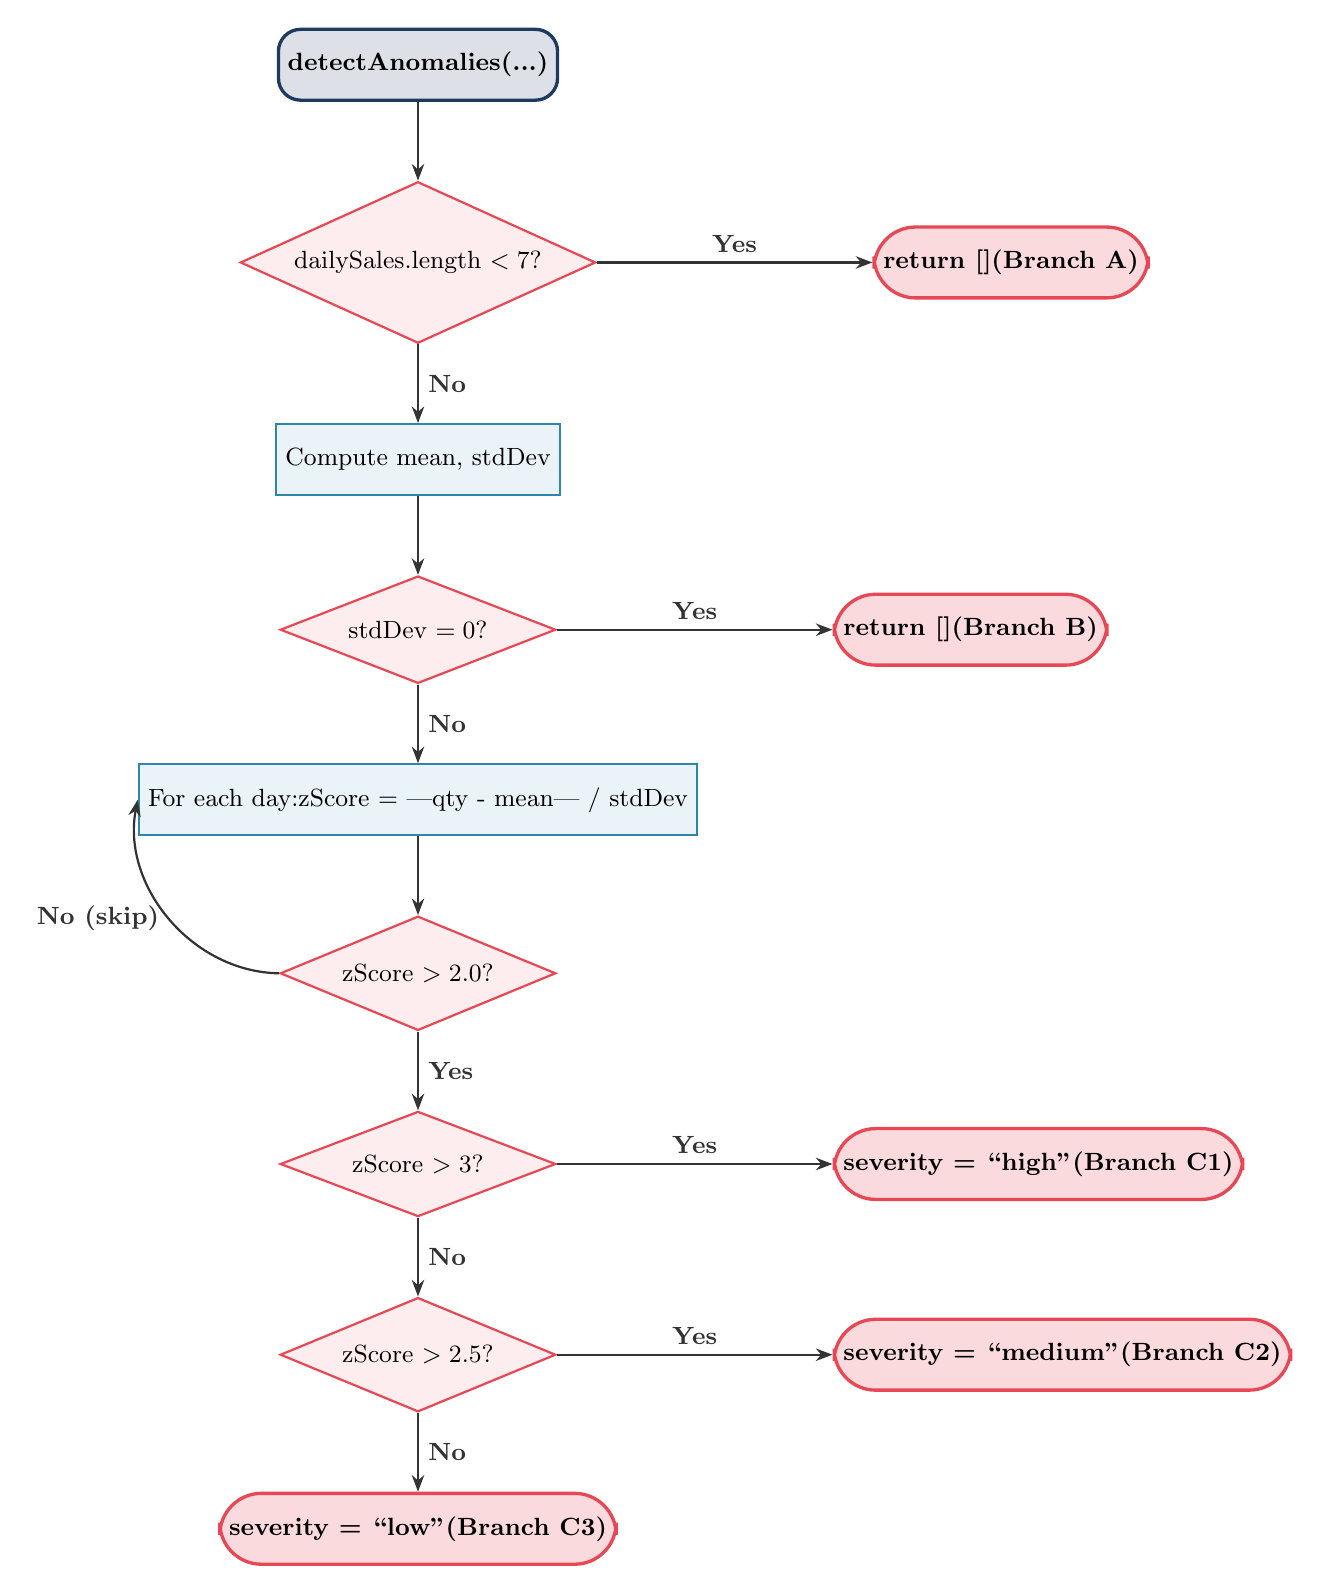
\begin{tikzpicture}[node distance=1.0cm]

  \node[startstop] (start) {detectAnomalies(...)};
  \node[decision, below=of start] (d1) {dailySales.length $< 7$?};
  \node[terminal, right=3.5cm of d1] (rA) {return [] \\ \small(Branch A)};
  \node[process, below=of d1] (stats) {Compute mean, stdDev};
  \node[decision, below=of stats] (d2) {stdDev $= 0$?};
  \node[terminal, right=3.5cm of d2] (rB) {return [] \\ \small(Branch B)};
  \node[process, below=of d2] (loop) {For each day: \\ zScore = |qty - mean| / stdDev};
  \node[decision, below=of loop] (d3) {zScore $> 2.0$?};
  \node[decision, below=of d3] (d4) {zScore $> 3$?};
  \node[terminal, right=3.5cm of d4] (rC1) {severity = ``high'' \\ \small(Branch C1)};
  \node[decision, below=of d4] (d5) {zScore $> 2.5$?};
  \node[terminal, right=3.5cm of d5] (rC2) {severity = ``medium'' \\ \small(Branch C2)};
  \node[terminal, below=of d5] (rC3) {severity = ``low'' \\ \small(Branch C3)};

  \draw[arrow] (start) -- (d1);
  \draw[arrow] (d1) -- node[yes, above]{Yes} (rA);
  \draw[arrow] (d1) -- node[no, right]{No} (stats);
  \draw[arrow] (stats) -- (d2);
  \draw[arrow] (d2) -- node[yes, above]{Yes} (rB);
  \draw[arrow] (d2) -- node[no, right]{No} (loop);
  \draw[arrow] (loop) -- (d3);
  \draw[arrow] (d3.west) to[bend left=50] node[no, left]{No (skip)} (loop.west);
  \draw[arrow] (d3) -- node[yes, right]{Yes} (d4);
  \draw[arrow] (d4) -- node[yes, above]{Yes} (rC1);
  \draw[arrow] (d4) -- node[no, right]{No} (d5);
  \draw[arrow] (d5) -- node[yes, above]{Yes} (rC2);
  \draw[arrow] (d5) -- node[no, right]{No} (rC3);

\end{tikzpicture}
\caption{detectAnomalies control flow with severity branches}
\end{figure}

\section{Reorder Recommendation Decision Diagram}

\begin{figure}[h!]
\centering
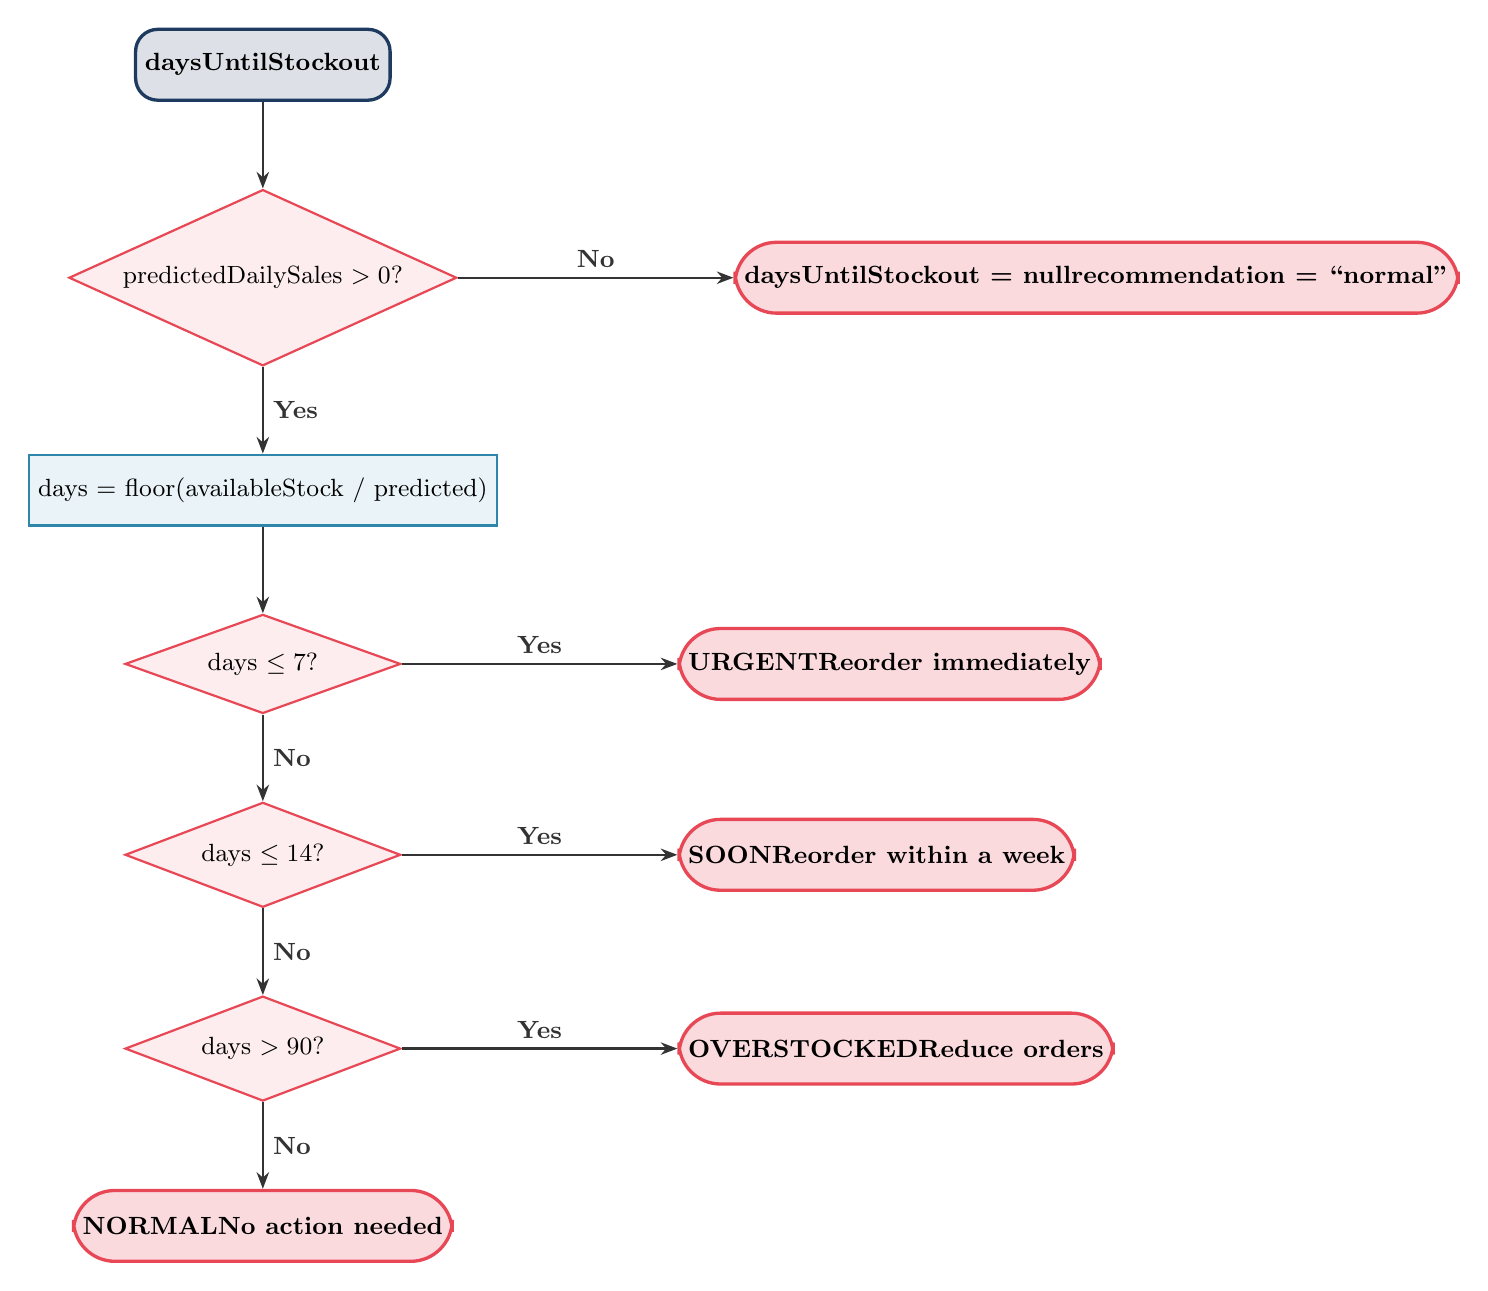
\begin{tikzpicture}[node distance=1.1cm]

  \node[startstop] (start) {daysUntilStockout};
  \node[decision, below=of start] (d1) {predictedDailySales $> 0$?};
  \node[terminal, right=3.5cm of d1] (null) {daysUntilStockout = null \\ recommendation = ``normal''};
  \node[process, below=of d1] (calc) {days = floor(availableStock / predicted)};
  \node[decision, below=of calc] (d2) {days $\leq 7$?};
  \node[terminal, right=3.5cm of d2] (urgent) {\textbf{URGENT} \\ Reorder immediately};
  \node[decision, below=of d2] (d3) {days $\leq 14$?};
  \node[terminal, right=3.5cm of d3] (soon) {\textbf{SOON} \\ Reorder within a week};
  \node[decision, below=of d3] (d4) {days $> 90$?};
  \node[terminal, right=3.5cm of d4] (over) {\textbf{OVERSTOCKED} \\ Reduce orders};
  \node[terminal, below=of d4] (normal) {\textbf{NORMAL} \\ No action needed};

  \draw[arrow] (start) -- (d1);
  \draw[arrow] (d1) -- node[no, above]{No} (null);
  \draw[arrow] (d1) -- node[yes, right]{Yes} (calc);
  \draw[arrow] (calc) -- (d2);
  \draw[arrow] (d2) -- node[yes, above]{Yes} (urgent);
  \draw[arrow] (d2) -- node[no, right]{No} (d3);
  \draw[arrow] (d3) -- node[yes, above]{Yes} (soon);
  \draw[arrow] (d3) -- node[no, right]{No} (d4);
  \draw[arrow] (d4) -- node[yes, above]{Yes} (over);
  \draw[arrow] (d4) -- node[no, right]{No} (normal);

\end{tikzpicture}
\caption{Reorder recommendation decision tree with boundary values}
\end{figure}

\section{Test Cases --- Demand Forecasting}

\begin{tcolorbox}[testbox, title={FORE-001 \hfill \ptwo}]
\textbf{Function:} \texttt{calculateMovingAverage} \\
\textbf{Scenario:} Window larger than data length \\
\textbf{Input:} \texttt{values = [10, 20, 30]}, \texttt{window = 5} \\
\textbf{Expected:} \texttt{[10, 15, 20]} (partial windows used for early elements) \\
\textbf{Coverage:} \texttt{Math.max(0, i - window + 1)} branch for early indices
\end{tcolorbox}

\begin{tcolorbox}[testbox, title={FORE-004 \hfill \pone}]
\textbf{Function:} \texttt{calculateStdDev} \\
\textbf{Scenario:} Empty array \\
\textbf{Input:} \texttt{values = []} \\
\textbf{Expected:} \texttt{0} (early return branch) \\
\textbf{Coverage:} Empty array branch
\end{tcolorbox}

\begin{tcolorbox}[criticalbox, title={FORE-005 \hfill \pone\ --- Zero Variance}]
\textbf{Function:} \texttt{calculateStdDev} \\
\textbf{Scenario:} All identical values (zero variance) \\
\textbf{Input:} \texttt{values = [5, 5, 5, 5, 5]} \\
\textbf{Expected:} \texttt{0} \\
\textbf{Note:} Critical for anomaly detection --- if stdDev = 0, detectAnomalies returns \texttt{[]} \\
\textbf{Coverage:} Zero variance case
\end{tcolorbox}

\begin{tcolorbox}[testbox, title={FORE-007 \hfill \pone}]
\textbf{Function:} \texttt{analyzeTrend} \\
\textbf{Scenario:} Less than 7 data points \\
\textbf{Input:} 6 days of data \\
\textbf{Expected:} \texttt{\{ trend: "stable", percentageChange: 0, periodDays: 6 \}} \\
\textbf{Coverage:} Branch A (insufficient data)
\end{tcolorbox}

\begin{tcolorbox}[testbox, title={FORE-008 \hfill \pone\ --- Boundary}]
\textbf{Function:} \texttt{analyzeTrend} \\
\textbf{Scenario:} Exactly 7 data points (boundary value) \\
\textbf{Input:} 7 days of data with clear upward trend \\
\textbf{Expected:} \texttt{trend = "increasing"} (NOT blocked by \texttt{< 7} check) \\
\textbf{Coverage:} Boundary value (exactly 7)
\end{tcolorbox}

\begin{tcolorbox}[criticalbox, title={FORE-012 \hfill \pone\ --- Division by Zero}]
\textbf{Function:} \texttt{analyzeTrend} \\
\textbf{Scenario:} All zero sales (\texttt{avgY = 0}) \\
\textbf{Input:} 8 days of \texttt{quantity = 0} \\
\textbf{Internal:} \texttt{avgY = 0} $\to$ \texttt{percentageChange = 0} (division by zero protection) \\
\textbf{Expected:} \texttt{trend = "stable"}, \texttt{percentageChange = 0} \\
\textbf{Coverage:} Division by zero protection
\end{tcolorbox}

\begin{tcolorbox}[criticalbox, title={FORE-018 \hfill \pone\ --- Zero Sales Stockout}]
\textbf{Function:} \texttt{generateProductForecast} \\
\textbf{Scenario:} Zero predicted daily sales (no sales history) \\
\textbf{Input:} \texttt{dailySales = []} \\
\textbf{Internal:} \texttt{predictedDailySales = 0} $\to$ division by zero protection \\
\textbf{Expected:} \texttt{daysUntilStockout = null} (not \texttt{Infinity} or \texttt{NaN}) \\
\textbf{Coverage:} Division by zero protection in daysUntilStockout
\end{tcolorbox}

\begin{tcolorbox}[testbox, title={FORE-019 \hfill \pone}]
\textbf{Function:} \texttt{generateProductForecast} \\
\textbf{Scenario:} Urgent reorder (\texttt{daysUntilStockout = 5}) \\
\textbf{Input:} \texttt{availableStock=50}, \texttt{predictedDailySales=10} $\to$ days = 5 \\
\textbf{Expected:} \texttt{reorderRecommendation = "urgent"} ($5 \leq 7$) \\
\textbf{Coverage:} Urgent branch
\end{tcolorbox}

\begin{tcolorbox}[testbox, title={FORE-020 \hfill \pone\ --- Boundary}]
\textbf{Function:} \texttt{generateProductForecast} \\
\textbf{Scenario:} \texttt{daysUntilStockout = 7} (exactly at lead days boundary) \\
\textbf{Input:} \texttt{availableStock=70}, \texttt{predictedDailySales=10} $\to$ days = 7 \\
\textbf{Expected:} \texttt{reorderRecommendation = "urgent"} ($7 \leq 7$) \\
\textbf{Coverage:} Boundary value for urgent
\end{tcolorbox}

\begin{tcolorbox}[testbox, title={FORE-022 \hfill \ptwo}]
\textbf{Function:} \texttt{generateProductForecast} \\
\textbf{Scenario:} Overstocked (\texttt{daysUntilStockout = 91}) \\
\textbf{Input:} \texttt{availableStock=910}, \texttt{predictedDailySales=10} $\to$ days = 91 \\
\textbf{Expected:} \texttt{reorderRecommendation = "overstocked"} ($91 > 90$) \\
\textbf{Coverage:} Overstocked branch
\end{tcolorbox}

\begin{tcolorbox}[testbox, title={FORE-023 \hfill \ptwo\ --- Boundary}]
\textbf{Function:} \texttt{generateProductForecast} \\
\textbf{Scenario:} \texttt{daysUntilStockout = 90} (NOT overstocked) \\
\textbf{Input:} \texttt{availableStock=900}, \texttt{predictedDailySales=10} $\to$ days = 90 \\
\textbf{Expected:} \texttt{reorderRecommendation = "normal"} ($90$ is NOT $> 90$) \\
\textbf{Coverage:} Boundary value for overstocked
\end{tcolorbox}


% ══════════════════════════════════════════════════════════════════════════════
\chapter{Module 5: Email Notification System}
% ══════════════════════════════════════════════════════════════════════════════

\textbf{Source File:} \texttt{lib/email/notifications.ts}

\section{isLowStock \& isOutOfStock Logic}

\begin{tcolorbox}[infobox, title={Stock Alert Thresholds}]
\begin{itemize}
  \item \texttt{LOW\_STOCK\_THRESHOLD = 20}
  \item \texttt{isLowStock(qty, threshold=20):} \texttt{qty > 0 \&\& qty <= threshold}
  \item \texttt{isOutOfStock(qty):} \texttt{qty === 0} (strict equality)
\end{itemize}
\end{tcolorbox}

\subsection{isLowStock Truth Table}

\begin{center}
\begin{tabular}{rrlc}
  \toprule
  \textbf{quantity} & \textbf{threshold} & \textbf{Evaluation} & \textbf{Result} \\
  \midrule
  0  & 20 & $0 > 0$ is FALSE (short-circuit) & \texttt{false} \\
  1  & 20 & $1 > 0$ AND $1 \leq 20$          & \texttt{true} \\
  20 & 20 & $20 > 0$ AND $20 \leq 20$        & \texttt{true} \\
  21 & 20 & $21 > 0$ AND $21 \leq 20$ = FALSE & \texttt{false} \\
  $-1$ & 20 & $-1 > 0$ is FALSE (short-circuit) & \texttt{false} \\
  \bottomrule
\end{tabular}
\end{center}

\subsection{sendLowStockAlert Control Flow}

\begin{figure}[h!]
\centering
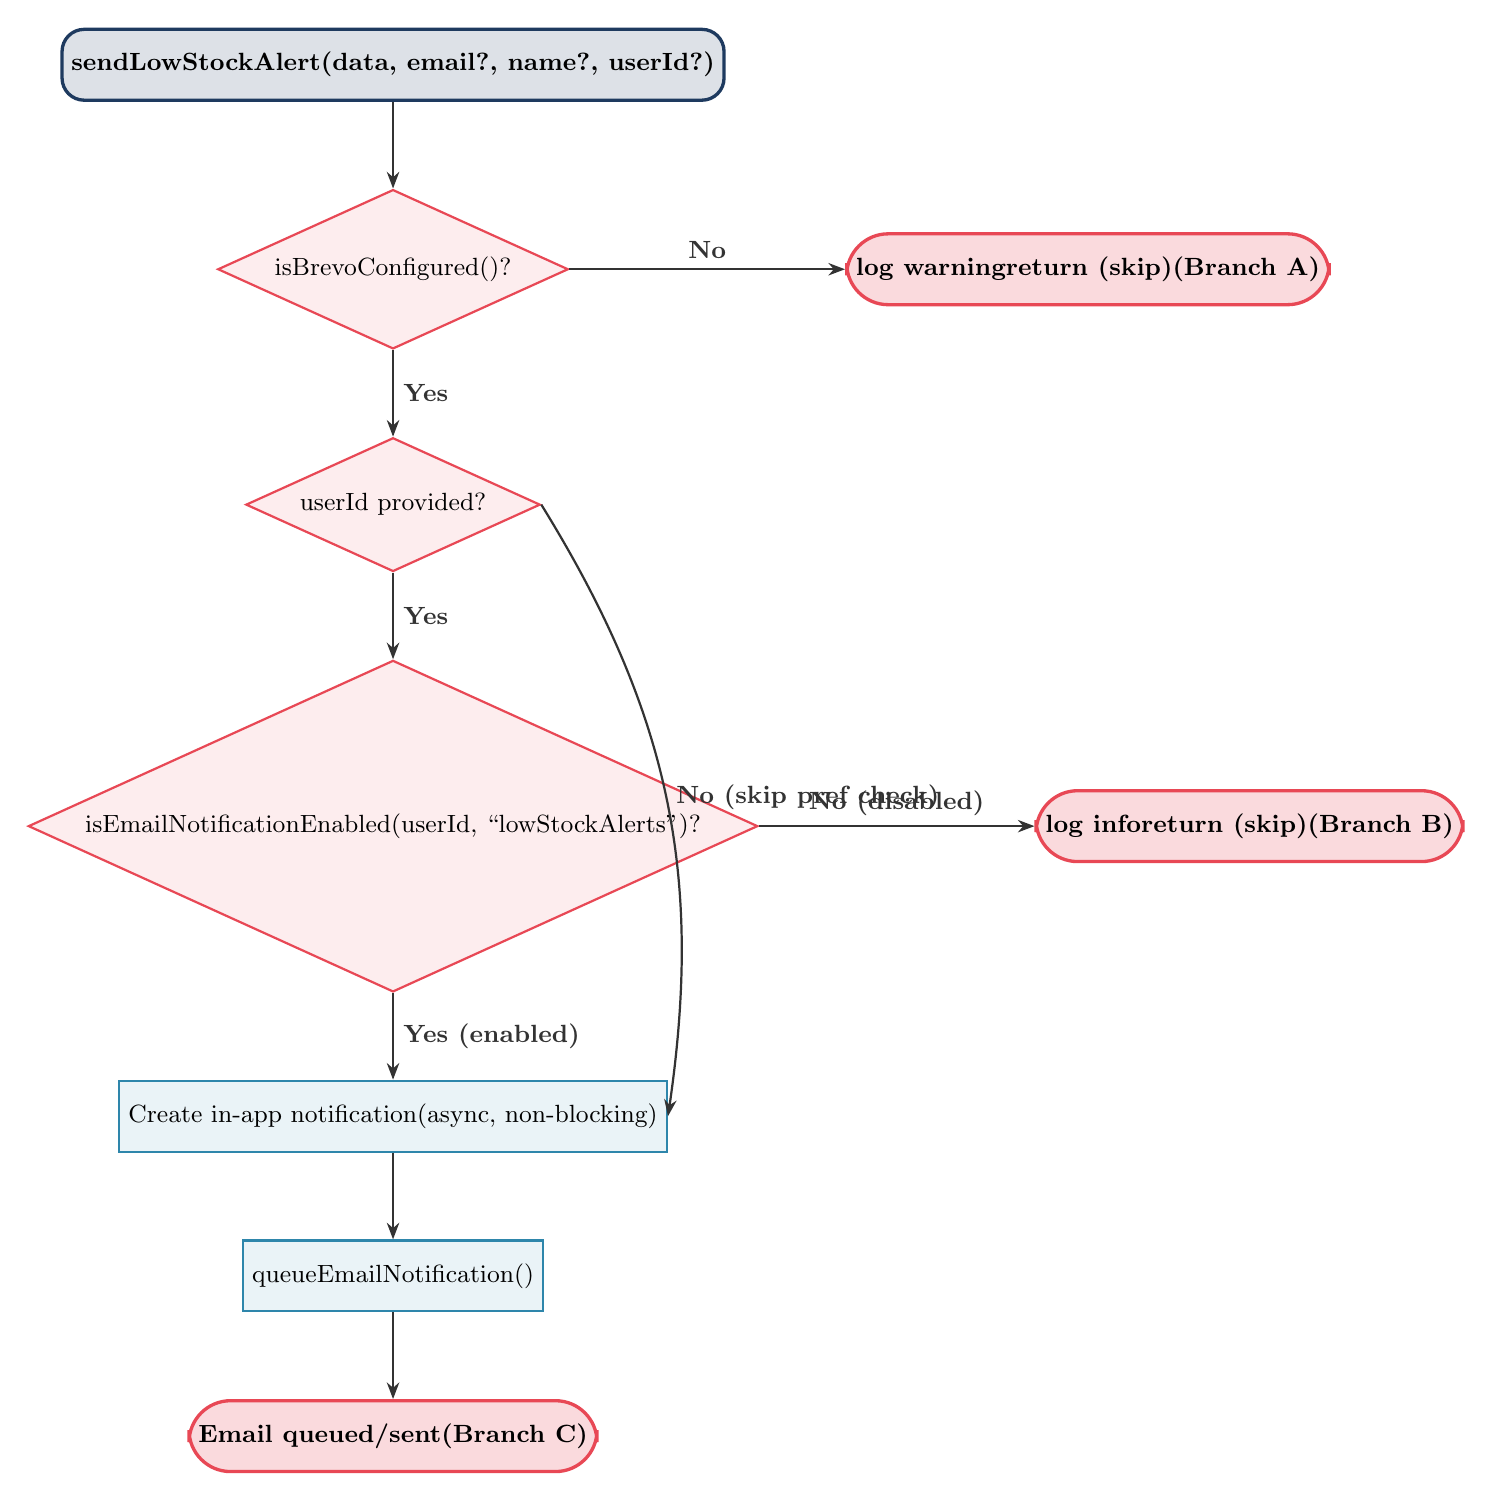
\begin{tikzpicture}[node distance=1.1cm]

  \node[startstop] (start) {sendLowStockAlert(data, email?, name?, userId?)};
  \node[decision, below=of start] (d1) {isBrevoConfigured()?};
  \node[terminal, right=3.5cm of d1] (rA) {log warning \\ return (skip) \\ \small(Branch A)};
  \node[decision, below=of d1] (d2) {userId provided?};
  \node[decision, below=of d2] (d3) {isEmailNotificationEnabled \\ (userId, ``lowStockAlerts'')?};
  \node[terminal, right=3.5cm of d3] (rB) {log info \\ return (skip) \\ \small(Branch B)};
  \node[process, below=of d3] (inapp) {Create in-app notification \\ (async, non-blocking)};
  \node[process, below=of inapp] (queue) {queueEmailNotification()};
  \node[terminal, below=of queue] (rC) {Email queued/sent \\ \small(Branch C)};

  \draw[arrow] (start) -- (d1);
  \draw[arrow] (d1) -- node[no, above]{No} (rA);
  \draw[arrow] (d1) -- node[yes, right]{Yes} (d2);
  \draw[arrow] (d2.east) to[bend left=20] node[no, right]{No (skip pref check)} (inapp.east);
  \draw[arrow] (d2) -- node[yes, right]{Yes} (d3);
  \draw[arrow] (d3) -- node[no, above]{No (disabled)} (rB);
  \draw[arrow] (d3) -- node[yes, right]{Yes (enabled)} (inapp);
  \draw[arrow] (inapp) -- (queue);
  \draw[arrow] (queue) -- (rC);

\end{tikzpicture}
\caption{sendLowStockAlert control flow with all branches}
\end{figure}

\section{Test Cases --- Email Notifications}

\begin{tcolorbox}[criticalbox, title={EMAIL-001 \hfill \pone\ --- Out of Stock Not Low Stock}]
\textbf{Function:} \texttt{isLowStock} \\
\textbf{Scenario:} Quantity is 0 (out of stock, not low stock) \\
\textbf{Input:} \texttt{quantity = 0}, \texttt{threshold = 20} \\
\textbf{Internal:} $0 > 0$ is \texttt{FALSE} $\to$ short-circuit $\to$ \texttt{return false} \\
\textbf{Expected:} \texttt{false} \\
\textbf{Coverage:} First condition false (AND short-circuit)
\end{tcolorbox}

\begin{tcolorbox}[testbox, title={EMAIL-002 \hfill \pone\ --- At Threshold Boundary}]
\textbf{Function:} \texttt{isLowStock} \\
\textbf{Scenario:} Quantity exactly at threshold \\
\textbf{Input:} \texttt{quantity = 20}, \texttt{threshold = 20} \\
\textbf{Internal:} $20 > 0$ AND $20 \leq 20$ $\to$ \texttt{true} \\
\textbf{Expected:} \texttt{true} \\
\textbf{Coverage:} Boundary value (at threshold)
\end{tcolorbox}

\begin{tcolorbox}[testbox, title={EMAIL-003 \hfill \pone\ --- Above Threshold}]
\textbf{Function:} \texttt{isLowStock} \\
\textbf{Scenario:} Quantity one above threshold \\
\textbf{Input:} \texttt{quantity = 21}, \texttt{threshold = 20} \\
\textbf{Internal:} $21 > 0$ AND $21 \leq 20$ $\to$ \texttt{false} \\
\textbf{Expected:} \texttt{false} \\
\textbf{Coverage:} Boundary value + 1
\end{tcolorbox}

\begin{tcolorbox}[testbox, title={EMAIL-007 \hfill \pone}]
\textbf{Function:} \texttt{isOutOfStock} \\
\textbf{Scenario:} Quantity is exactly 0 \\
\textbf{Input:} \texttt{quantity = 0} \\
\textbf{Internal:} \texttt{0 === 0} $\to$ \texttt{true} \\
\textbf{Expected:} \texttt{true} \\
\textbf{Coverage:} Exact zero match
\end{tcolorbox}

\begin{tcolorbox}[testbox, title={EMAIL-009 \hfill \ptwo}]
\textbf{Function:} \texttt{isOutOfStock} \\
\textbf{Scenario:} Negative quantity (corrupted data) \\
\textbf{Input:} \texttt{quantity = -1} \\
\textbf{Internal:} \texttt{-1 === 0} is \texttt{false} (strict equality) \\
\textbf{Expected:} \texttt{false} \\
\textbf{Coverage:} Strict equality check
\end{tcolorbox}

\begin{tcolorbox}[testbox, title={EMAIL-010 \hfill \pone}]
\textbf{Function:} \texttt{sendLowStockAlert} \\
\textbf{Scenario:} Brevo not configured \\
\textbf{Mock:} \texttt{isBrevoConfigured()} returns \texttt{false} \\
\textbf{Expected:} Function returns early, no email sent, warning logged \\
\textbf{Coverage:} Branch A
\end{tcolorbox}

\begin{tcolorbox}[testbox, title={EMAIL-011 \hfill \ptwo}]
\textbf{Function:} \texttt{sendLowStockAlert} \\
\textbf{Scenario:} User has disabled low stock alerts \\
\textbf{Mock:} \texttt{isBrevoConfigured()} = \texttt{true}; \texttt{isEmailNotificationEnabled} = \texttt{false} \\
\textbf{Expected:} Function returns early, no email sent, info logged \\
\textbf{Coverage:} Branch B
\end{tcolorbox}

% ══════════════════════════════════════════════════════════════════════════════
\chapter{Module 6: Rate Limiting \& Caching}
% ══════════════════════════════════════════════════════════════════════════════

\textbf{Source File:} \texttt{lib/api/rate-limit.ts}

\section{Rate Limit Configurations}

\begin{center}
\begin{tabular}{lccp{6cm}}
  \toprule
  \textbf{Config} & \textbf{Limit} & \textbf{Window} & \textbf{Identifier} \\
  \midrule
  \texttt{standard} & 600 req & 60 sec & User ID (header) or IP \\
  \texttt{strict}   & 10 req  & 60 sec & User ID (header) or IP \\
  \texttt{auth}     & 5 req   & 60 sec & \textbf{Always IP} (brute-force protection) \\
  \bottomrule
\end{tabular}
\end{center}

\subsection{Identifier Resolution Flowchart}

\begin{figure}[h!]
\centering
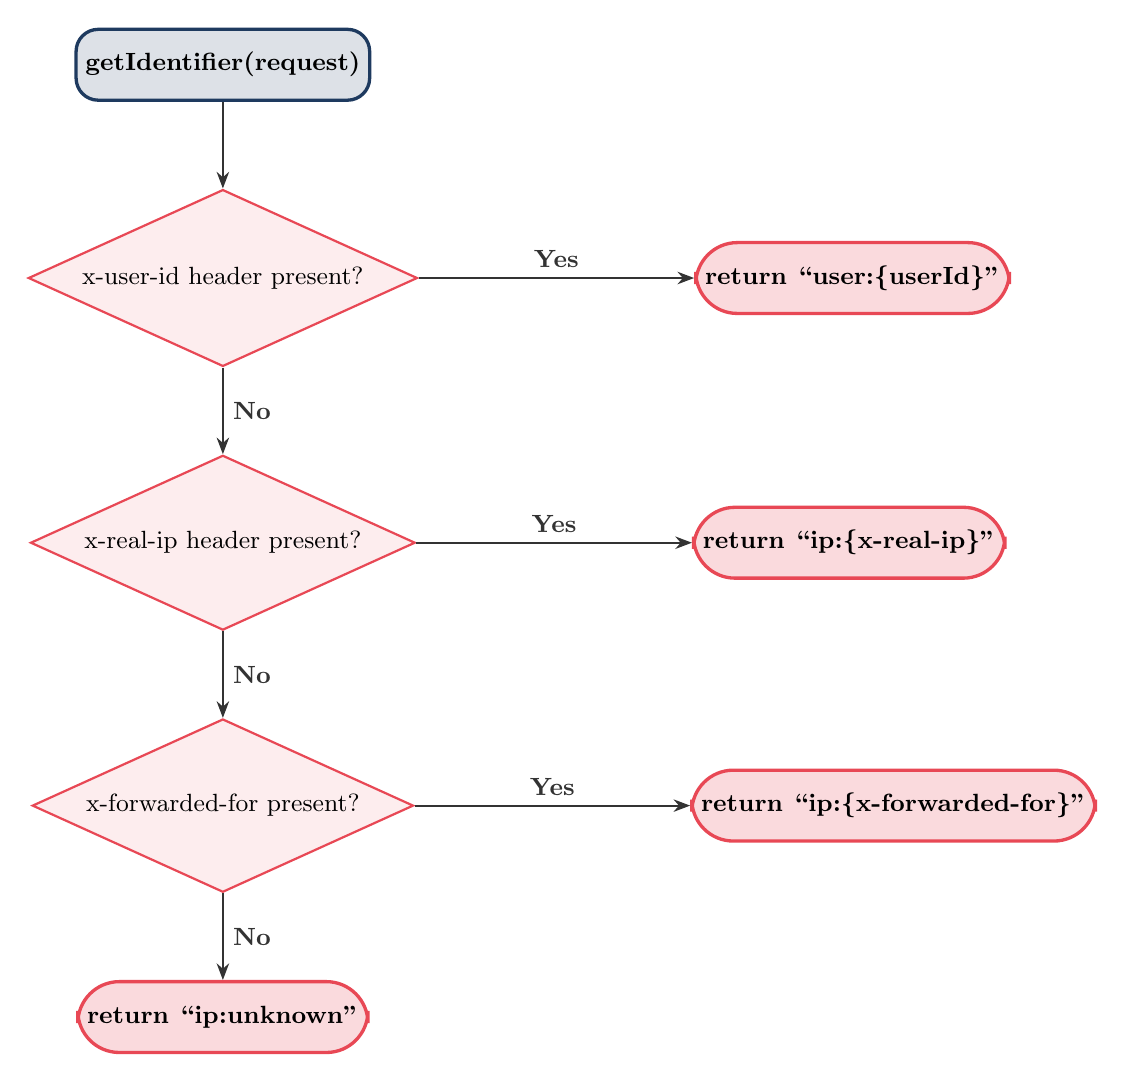
\begin{tikzpicture}[node distance=1.1cm]

  \node[startstop] (start) {getIdentifier(request)};
  \node[decision, below=of start] (d1) {x-user-id header present?};
  \node[terminal, right=3.5cm of d1] (uid) {return ``user:\{userId\}''};
  \node[decision, below=of d1] (d2) {x-real-ip header present?};
  \node[terminal, right=3.5cm of d2] (rip) {return ``ip:\{x-real-ip\}''};
  \node[decision, below=of d2] (d3) {x-forwarded-for present?};
  \node[terminal, right=3.5cm of d3] (fwd) {return ``ip:\{x-forwarded-for\}''};
  \node[terminal, below=of d3] (unk) {return ``ip:unknown''};

  \draw[arrow] (start) -- (d1);
  \draw[arrow] (d1) -- node[yes, above]{Yes} (uid);
  \draw[arrow] (d1) -- node[no, right]{No} (d2);
  \draw[arrow] (d2) -- node[yes, above]{Yes} (rip);
  \draw[arrow] (d2) -- node[no, right]{No} (d3);
  \draw[arrow] (d3) -- node[yes, above]{Yes} (fwd);
  \draw[arrow] (d3) -- node[no, right]{No} (unk);

\end{tikzpicture}
\caption{Rate limit identifier resolution (standard/strict configs)}
\end{figure}

\section{Test Cases --- Rate Limiting}

\begin{tcolorbox}[criticalbox, title={RATE-005 \hfill \pone\ --- Auth Always Uses IP}]
\textbf{Config:} \texttt{defaultRateLimits.auth} \\
\textbf{Scenario:} Auth endpoint always uses IP even if user ID header present \\
\textbf{Input:} Request with \texttt{x-user-id = "user123"} AND \texttt{x-real-ip = "1.2.3.4"} \\
\textbf{Expected:} \texttt{"ip:1.2.3.4"} (NOT \texttt{"user:user123"}) \\
\textbf{Coverage:} Auth always-IP security requirement
\end{tcolorbox}

\begin{tcolorbox}[testbox, title={RATE-007 \hfill \pone}]
\textbf{Function:} \texttt{withRateLimit} \\
\textbf{Scenario:} Rate limit exceeded \\
\textbf{Mock:} \texttt{checkRateLimit} returns \texttt{\{ limited: true, retryAfter: 30 \}} \\
\textbf{Expected:} Returns \texttt{NextResponse} with status \textbf{429} and \texttt{Retry-After} header \\
\textbf{Coverage:} Rate limited branch
\end{tcolorbox}

% ══════════════════════════════════════════════════════════════════════════════
\chapter{Module 7: Input Validation (Zod Schemas)}
% ══════════════════════════════════════════════════════════════════════════════

\section{Validation Behaviour}

\begin{tcolorbox}[infobox, title={Zod Schema Behaviour}]
When \texttt{schema.parse(data)} is called:
\begin{itemize}
  \item \textbf{Valid data:} Returns typed, parsed data object.
  \item \textbf{Invalid data:} Throws \texttt{ZodError} with field-level error messages.
\end{itemize}
The login route catches \texttt{ZodError} and returns HTTP 400.
\end{tcolorbox}

\section{Test Cases --- Input Validation}

\begin{tcolorbox}[testbox, title={VAL-002 \hfill \pone}]
\textbf{Schema:} \texttt{loginSchema} \\
\textbf{Scenario:} Invalid email format \\
\textbf{Input:} \texttt{\{ email: "not-an-email", password: "pass123" \}} \\
\textbf{Expected:} \texttt{ZodError} thrown, error on \texttt{"email"} field \\
\textbf{Coverage:} Email format validation
\end{tcolorbox}

\begin{tcolorbox}[criticalbox, title={VAL-006 \hfill \pone\ --- Zero Quantity}]
\textbf{Schema:} \texttt{createOrderSchema} \\
\textbf{Scenario:} Item with \texttt{quantity = 0} \\
\textbf{Input:} \texttt{\{ items: [\{ productId: "abc", quantity: 0 \}] \}} \\
\textbf{Expected:} \texttt{ZodError} (if \texttt{min(1)} enforced on quantity) \\
\textbf{Coverage:} Zero quantity validation
\end{tcolorbox}

\begin{tcolorbox}[criticalbox, title={VAL-012 \hfill \pone\ --- Injection Attempt}]
\textbf{Scenario:} NoSQL injection attempt in email field \\
\textbf{Input:} \texttt{\{ email: "\$where: function() \{ return true; \}" \}} \\
\textbf{Expected:} \texttt{ZodError} (invalid email format) or safely stored as string \\
\textbf{Note:} MongoDB is not SQL-injectable, but Zod should reject invalid emails \\
\textbf{Coverage:} Injection attempt handling
\end{tcolorbox}

\begin{tcolorbox}[criticalbox, title={VAL-013 \hfill \pone\ --- XSS Attempt}]
\textbf{Scenario:} XSS attempt in notes field \\
\textbf{Input:} \texttt{\{ notes: "<script>alert('xss')</script>" \}} \\
\textbf{Expected:} Stored as plain string (no execution), or sanitized \\
\textbf{Coverage:} XSS in text fields
\end{tcolorbox}


% ══════════════════════════════════════════════════════════════════════════════
\chapter{Module 8: Role-Based Access Control (RBAC)}
% ══════════════════════════════════════════════════════════════════════════════

\section{RBAC Decision Flowchart}

\begin{figure}[h!]
\centering
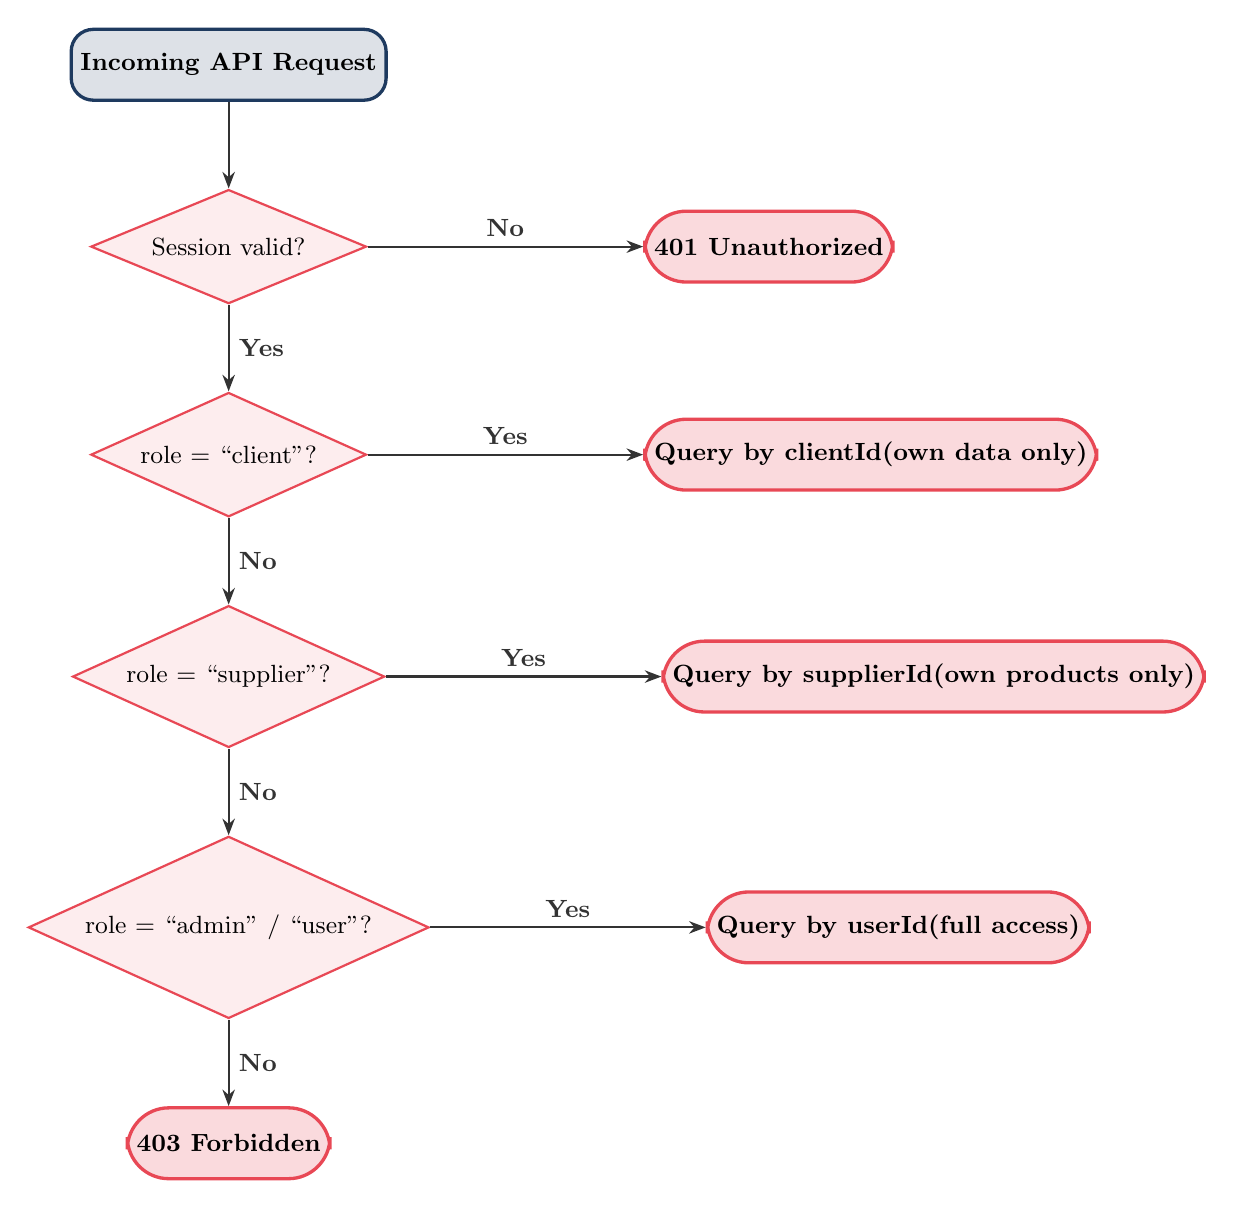
\begin{tikzpicture}[node distance=1.1cm]

  \node[startstop] (start) {Incoming API Request};
  \node[decision, below=of start] (d1) {Session valid?};
  \node[terminal, right=3.5cm of d1] (r401) {401 Unauthorized};
  \node[decision, below=of d1] (d2) {role = ``client''?};
  \node[terminal, right=3.5cm of d2] (client) {Query by clientId \\ (own data only)};
  \node[decision, below=of d2] (d3) {role = ``supplier''?};
  \node[terminal, right=3.5cm of d3] (supplier) {Query by supplierId \\ (own products only)};
  \node[decision, below=of d3] (d4) {role = ``admin'' / ``user''?};
  \node[terminal, right=3.5cm of d4] (admin) {Query by userId \\ (full access)};
  \node[terminal, below=of d4] (r403) {403 Forbidden};

  \draw[arrow] (start) -- (d1);
  \draw[arrow] (d1) -- node[no, above]{No} (r401);
  \draw[arrow] (d1) -- node[yes, right]{Yes} (d2);
  \draw[arrow] (d2) -- node[yes, above]{Yes} (client);
  \draw[arrow] (d2) -- node[no, right]{No} (d3);
  \draw[arrow] (d3) -- node[yes, above]{Yes} (supplier);
  \draw[arrow] (d3) -- node[no, right]{No} (d4);
  \draw[arrow] (d4) -- node[yes, above]{Yes} (admin);
  \draw[arrow] (d4) -- node[no, right]{No} (r403);

\end{tikzpicture}
\caption{RBAC decision flow for API routes}
\end{figure}

\section{Test Cases --- RBAC}

\begin{tcolorbox}[criticalbox, title={RBAC-008 \hfill \pone\ --- Unauthenticated}]
\textbf{Scenario:} Unauthenticated request to any protected route \\
\textbf{Mock:} \texttt{getSessionFromRequest} returns \texttt{null} \\
\textbf{Expected:} \textbf{401 Unauthorized} response \\
\textbf{Coverage:} Auth guard (all routes)
\end{tcolorbox}

\begin{tcolorbox}[criticalbox, title={RBAC-010 \hfill \pone\ --- Data Isolation}]
\textbf{Scenario:} Supplier tries to access another supplier's products \\
\textbf{Mock:} \texttt{session.role = "supplier"}, \texttt{supplierId = "supplierA"} \\
\textbf{Expected:} Only products with \texttt{supplierId = "supplierA"} returned \\
\textbf{Coverage:} Data isolation between suppliers
\end{tcolorbox}

\begin{tcolorbox}[criticalbox, title={RBAC-011 \hfill \pone\ --- Horizontal Privilege Escalation}]
\textbf{Scenario:} User tries to access another user's orders \\
\textbf{Mock:} \texttt{session.id = "userA"}, request attempts to get orders for \texttt{"userB"} \\
\textbf{Expected:} Only userA's orders returned (userId from session, not request body) \\
\textbf{Coverage:} Horizontal privilege escalation prevention
\end{tcolorbox}

% ══════════════════════════════════════════════════════════════════════════════
\chapter{Module 9: Data Integrity \& Database Layer}
% ══════════════════════════════════════════════════════════════════════════════

\section{Unique Constraints}

\begin{center}
\begin{tabular}{lll}
  \toprule
  \textbf{Model} & \textbf{Field} & \textbf{Constraint} \\
  \midrule
  \texttt{User}    & \texttt{email}         & Globally unique \\
  \texttt{Product} & \texttt{sku}           & Globally unique \\
  \texttt{Order}   & \texttt{orderNumber}   & Globally unique \\
  \texttt{Invoice} & \texttt{invoiceNumber} & Globally unique \\
  \texttt{Invoice} & \texttt{orderId}       & Unique (one invoice per order) \\
  \bottomrule
\end{tabular}
\end{center}

\section{Cascade Relationships}

\begin{center}
\begin{tabular}{lll}
  \toprule
  \textbf{Parent} & \textbf{Child} & \textbf{On Delete} \\
  \midrule
  \texttt{Order}         & \texttt{Invoice}   & Cascade (invoice deleted) \\
  \texttt{Order}         & \texttt{OrderItem} & Cascade (items deleted) \\
  \texttt{User}          & \texttt{Notification} & Cascade \\
  \texttt{SupportTicket} & \texttt{SupportTicketReply} & Cascade \\
  \bottomrule
\end{tabular}
\end{center}

\section{Test Cases --- Data Integrity}

\begin{tcolorbox}[criticalbox, title={DB-004 \hfill \pone\ --- Cascade Delete}]
\textbf{Scenario:} Deleting an order removes its invoice \\
\textbf{Steps:} (1) Create order \quad (2) Create invoice for that order \quad (3) Delete the order \\
\textbf{Expected:} Invoice is also deleted (cascade) \\
\textbf{Coverage:} \texttt{onDelete: Cascade} relationship
\end{tcolorbox}

\begin{tcolorbox}[criticalbox, title={DB-007 \hfill \pone\ --- Atomicity Gap}]
\textbf{Scenario:} \texttt{prisma.product.update} fails after \texttt{order.create} succeeds \\
\textbf{Expected:} Order exists but stock not reserved (partial state) \\
\textbf{Note:} \textbf{Known issue} --- order creation is not wrapped in a database transaction. \\
This is a documented architectural risk. \\
\textbf{Coverage:} Transaction atomicity gap
\end{tcolorbox}

\begin{tcolorbox}[testbox, title={DB-008 \hfill \ptwo}]
\textbf{Scenario:} Audit log failure does not break main operation \\
\textbf{Mock:} \texttt{createAuditLog} throws an error \\
\textbf{Expected:} Main operation (order create, etc.) still succeeds \\
\textbf{Coverage:} Audit log error isolation (fire-and-forget)
\end{tcolorbox}

% ══════════════════════════════════════════════════════════════════════════════
\chapter{Module 10: Stripe Payment \& Webhook Handling}
% ══════════════════════════════════════════════════════════════════════════════

\section{Webhook Security Flow}

\begin{figure}[h!]
\centering
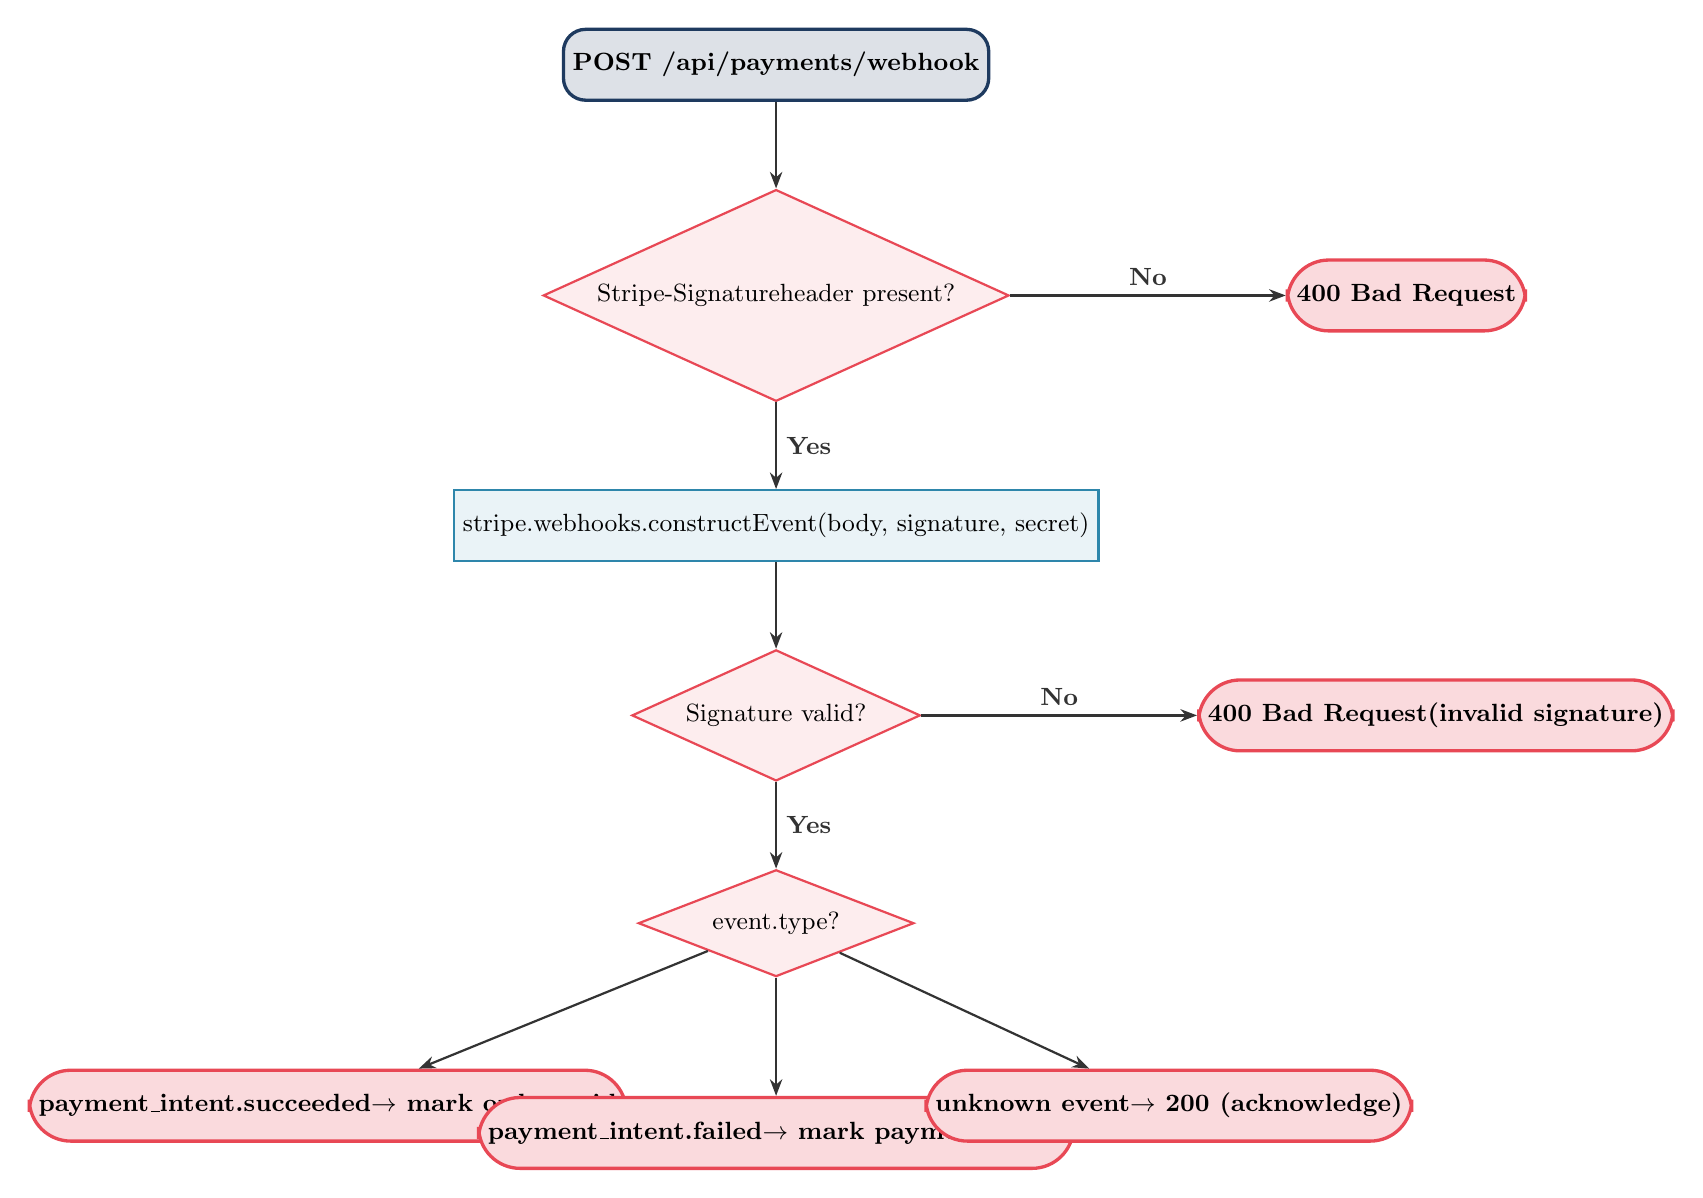
\begin{tikzpicture}[node distance=1.1cm]

  \node[startstop] (start) {POST /api/payments/webhook};
  \node[decision, below=of start] (d1) {Stripe-Signature \\ header present?};
  \node[terminal, right=3.5cm of d1] (r400a) {400 Bad Request};
  \node[process, below=of d1] (verify) {stripe.webhooks.constructEvent \\ (body, signature, secret)};
  \node[decision, below=of verify] (d2) {Signature valid?};
  \node[terminal, right=3.5cm of d2] (r400b) {400 Bad Request \\ (invalid signature)};
  \node[decision, below=of d2] (d3) {event.type?};
  \node[terminal, below left=1.5cm and 1cm of d3] (paid) {payment\_intent.succeeded \\ $\to$ mark order paid};
  \node[terminal, below=1.5cm of d3] (failed) {payment\_intent.failed \\ $\to$ mark payment failed};
  \node[terminal, below right=1.5cm and 1cm of d3] (other) {unknown event \\ $\to$ 200 (acknowledge)};

  \draw[arrow] (start) -- (d1);
  \draw[arrow] (d1) -- node[no, above]{No} (r400a);
  \draw[arrow] (d1) -- node[yes, right]{Yes} (verify);
  \draw[arrow] (verify) -- (d2);
  \draw[arrow] (d2) -- node[no, above]{No} (r400b);
  \draw[arrow] (d2) -- node[yes, right]{Yes} (d3);
  \draw[arrow] (d3) -- (paid);
  \draw[arrow] (d3) -- (failed);
  \draw[arrow] (d3) -- (other);

\end{tikzpicture}
\caption{Stripe webhook security and event handling flow}
\end{figure}

\section{Test Cases --- Stripe Payments}

\begin{tcolorbox}[criticalbox, title={PAY-001 \hfill \pone\ --- Invalid Signature}]
\textbf{Scenario:} Webhook with invalid signature \\
\textbf{Input:} Valid body but wrong \texttt{Stripe-Signature} header \\
\textbf{Expected:} \texttt{stripe.webhooks.constructEvent} throws $\to$ \textbf{400} response \\
\textbf{Coverage:} Signature verification failure branch
\end{tcolorbox}

\begin{tcolorbox}[criticalbox, title={PAY-002 \hfill \pone\ --- Missing Signature}]
\textbf{Scenario:} Webhook with no \texttt{Stripe-Signature} header \\
\textbf{Expected:} \textbf{400} response (cannot verify) \\
\textbf{Coverage:} Missing signature branch
\end{tcolorbox}

\begin{tcolorbox}[testbox, title={PAY-005 \hfill \ptwo}]
\textbf{Scenario:} Unknown webhook event type \\
\textbf{Mock:} \texttt{event.type = "some.unknown.event"} \\
\textbf{Expected:} Event ignored gracefully, \textbf{200} response (acknowledge receipt) \\
\textbf{Coverage:} Unknown event type branch
\end{tcolorbox}


% ══════════════════════════════════════════════════════════════════════════════
\chapter{Complete Test Case Matrix}
% ══════════════════════════════════════════════════════════════════════════════

\section{Authentication Tests}

\begin{longtable}{p{2cm}p{3.5cm}p{5cm}p{1.5cm}c}
  \toprule
  \textbf{Test ID} & \textbf{Function} & \textbf{Scenario} & \textbf{Coverage} & \textbf{Pri.} \\
  \midrule
  \endhead
  \testid{AUTH-001} & verifyToken & Empty string token & Branch A & \pone \\
  \testid{AUTH-002} & verifyToken & String ``null'' token & Branch A & \pone \\
  \testid{AUTH-003} & verifyToken & String ``undefined'' token & Branch A & \pone \\
  \testid{AUTH-004} & verifyToken & Valid JWT & Branch E & \pone \\
  \testid{AUTH-005} & verifyToken & Expired JWT & Exception & \pone \\
  \testid{AUTH-006} & verifyToken & Wrong secret & Security & \pone \\
  \testid{AUTH-007} & verifyToken & Malformed token & Exception & \pone \\
  \testid{AUTH-008} & generateToken & Payload integrity & Statement & \pone \\
  \testid{AUTH-009} & hashPassword + compare & Round-trip hash & Statement & \pone \\
  \testid{AUTH-010} & comparePassword & Wrong password & Branch & \pone \\
  \testid{AUTH-011} & POST /login & Missing email & Validation & \pone \\
  \testid{AUTH-012} & POST /login & User not found & Branch & \pone \\
  \testid{AUTH-013} & POST /login & Corrupted user data & Branch & \ptwo \\
  \testid{AUTH-014} & POST /login & Correct credentials & Statement & \pone \\
  \testid{AUTH-015} & getSession & No cookie & Branch & \pone \\
  \testid{AUTH-016} & getSession & Deleted user & Branch & \ptwo \\
  \bottomrule
\end{longtable}

\section{Order Management Tests}

\begin{longtable}{p{2cm}p{3.5cm}p{5cm}p{1.5cm}c}
  \toprule
  \textbf{Test ID} & \textbf{Function} & \textbf{Scenario} & \textbf{Coverage} & \textbf{Pri.} \\
  \midrule
  \endhead
  \testid{ORD-001} & generateOrderNumber & First order of day & Statement & \ptwo \\
  \testid{ORD-002} & generateOrderNumber & 9999 orders today & Boundary & \pthree \\
  \testid{ORD-003} & createOrder & Product not found & Branch & \pone \\
  \testid{ORD-004} & createOrder & Insufficient stock & Branch & \pone \\
  \testid{ORD-005} & createOrder & Exact stock match & Boundary & \pone \\
  \testid{ORD-006} & createOrder & Boundary + 1 & Boundary & \pone \\
  \testid{ORD-007} & createOrder & Null reservedQty & Branch & \ptwo \\
  \testid{ORD-008} & createOrder & Partial failure & Atomicity & \pone \\
  \testid{ORD-009} & createOrder & Total calculation & Statement & \pone \\
  \testid{ORD-010} & createOrder & Zero tax/shipping & Branch & \ptwo \\
  \testid{ORD-011} & createOrder & Stock reservation & Side-effect & \pone \\
  \testid{ORD-012} & GET /orders & Unauthenticated & Security & \pone \\
  \testid{ORD-013} & GET /orders & Supplier no record & Branch & \ptwo \\
  \testid{ORD-014} & GET /orders & Cache hit & Statement & \ptwo \\
  \testid{ORD-015} & GET /orders & Client role & Branch & \pone \\
  \testid{ORD-016} & GET /orders & Rate limited & Branch & \ptwo \\
  \bottomrule
\end{longtable}

\section{Invoice Tests}

\begin{longtable}{p{2cm}p{3.5cm}p{5cm}p{1.5cm}c}
  \toprule
  \textbf{Test ID} & \textbf{Function} & \textbf{Scenario} & \textbf{Coverage} & \textbf{Pri.} \\
  \midrule
  \endhead
  \testid{INV-001} & generateInvoiceNumber & No collision & Statement & \ptwo \\
  \testid{INV-002} & generateInvoiceNumber & Collision handling & Branch & \ptwo \\
  \testid{INV-003} & generateInvoiceNumber & Format structure & Statement & \ptwo \\
  \testid{INV-004} & createInvoice & Order not found & Branch & \pone \\
  \testid{INV-005} & createInvoice & Duplicate invoice & Branch & \pone \\
  \testid{INV-006} & createInvoice & Total calculation & Statement & \pone \\
  \testid{INV-007} & createInvoice & Negative total prevention & Branch & \pone \\
  \testid{INV-008} & createInvoice & Explicit zero tax & Branch & \ptwo \\
  \testid{INV-009} & createInvoice & Null tax fallback & Branch & \ptwo \\
  \testid{INV-010} & createInvoice & Double null fallback & Branch & \ptwo \\
  \testid{INV-011} & createInvoice & amountPaid = 0 & Statement & \pone \\
  \testid{INV-012} & createInvoice & Status = draft & Statement & \pone \\
  \testid{INV-013} & GET /invoices & Client role & Branch & \pone \\
  \testid{INV-014} & GET /invoices & Multi-status filter & Statement & \ptwo \\
  \testid{INV-015} & GET /invoices & No status filter & Branch & \ptwo \\
  \bottomrule
\end{longtable}

\section{Demand Forecasting Tests}

\begin{longtable}{p{2cm}p{3.5cm}p{5cm}p{1.5cm}c}
  \toprule
  \textbf{Test ID} & \textbf{Function} & \textbf{Scenario} & \textbf{Coverage} & \textbf{Pri.} \\
  \midrule
  \endhead
  \testid{FORE-001} & calculateMovingAverage & Window $>$ data length & Branch & \ptwo \\
  \testid{FORE-002} & calculateMovingAverage & Window = 1 & Boundary & \ptwo \\
  \testid{FORE-003} & calculateMovingAverage & Empty array & Boundary & \ptwo \\
  \testid{FORE-004} & calculateStdDev & Empty array & Branch & \pone \\
  \testid{FORE-005} & calculateStdDev & All identical values & Statement & \pone \\
  \testid{FORE-006} & calculateStdDev & Known values & Statement & \pone \\
  \testid{FORE-007} & analyzeTrend & $< 7$ data points & Branch A & \pone \\
  \testid{FORE-008} & analyzeTrend & Exactly 7 points & Boundary & \pone \\
  \testid{FORE-009} & analyzeTrend & Increasing trend & Branch B1 & \pone \\
  \testid{FORE-010} & analyzeTrend & Decreasing trend & Branch B2 & \pone \\
  \testid{FORE-011} & analyzeTrend & Stable trend & Branch B3 & \pone \\
  \testid{FORE-012} & analyzeTrend & All zero sales & Branch & \pone \\
  \testid{FORE-013} & detectAnomalies & $< 7$ points & Branch A & \pone \\
  \testid{FORE-014} & detectAnomalies & stdDev = 0 & Branch B & \pone \\
  \testid{FORE-015} & detectAnomalies & High severity spike & Branch C1 & \pone \\
  \testid{FORE-016} & detectAnomalies & Medium severity & Branch C2 & \ptwo \\
  \testid{FORE-017} & detectAnomalies & Low severity & Branch C3 & \ptwo \\
  \testid{FORE-018} & generateProductForecast & Zero sales (no crash) & Branch & \pone \\
  \testid{FORE-019} & generateProductForecast & Urgent reorder & Branch & \pone \\
  \testid{FORE-020} & generateProductForecast & Urgent boundary (=7) & Boundary & \pone \\
  \testid{FORE-021} & generateProductForecast & Soon boundary (=8) & Boundary & \pone \\
  \testid{FORE-022} & generateProductForecast & Overstocked ($>$90) & Branch & \ptwo \\
  \testid{FORE-023} & generateProductForecast & Not overstocked (=90) & Boundary & \ptwo \\
  \testid{FORE-024} & generateProductForecast & Max confidence score & Statement & \pthree \\
  \testid{FORE-025} & generateProductForecast & Min confidence score & Statement & \pthree \\
  \testid{FORE-026} & generateProductForecast & Weighted average & Statement & \ptwo \\
  \testid{FORE-027} & generateProductForecast & Fallback to overall avg & Branch & \ptwo \\
  \bottomrule
\end{longtable}

\section{Summary Statistics}

\begin{center}
\begin{tabular}{lrr}
  \toprule
  \textbf{Module} & \textbf{Test Cases} & \textbf{P1 Critical} \\
  \midrule
  Authentication          & 16 & 13 \\
  Order Management        & 16 & 10 \\
  Invoice Generation      & 15 &  8 \\
  Demand Forecasting      & 27 & 15 \\
  Email Notifications     & 13 &  6 \\
  Rate Limiting           &  8 &  4 \\
  Input Validation        & 15 &  7 \\
  RBAC                    & 11 &  9 \\
  Data Integrity          & 10 &  5 \\
  Stripe Payments         &  7 &  4 \\
  \midrule
  \textbf{TOTAL}          & \textbf{138} & \textbf{81} \\
  \bottomrule
\end{tabular}
\end{center}


% ══════════════════════════════════════════════════════════════════════════════
\chapter{Code Coverage Requirements}
% ══════════════════════════════════════════════════════════════════════════════

\section{Coverage Targets by Module}

\begin{center}
\begin{tabular}{lcccc}
  \toprule
  \textbf{Module / File} & \textbf{Statement} & \textbf{Branch} & \textbf{Function} & \textbf{Line} \\
  \midrule
  \texttt{utils/auth.ts}                  & 100\% & 100\% & 100\% & 100\% \\
  \texttt{lib/forecasting/demand-forecast} & 100\% & 100\% & 100\% & 100\% \\
  \texttt{lib/email/notifications.ts}      &  95\% & 100\% & 100\% &  95\% \\
  \texttt{lib/api/rate-limit.ts}           & 100\% & 100\% & 100\% & 100\% \\
  \texttt{lib/validations/}               &  95\% &  95\% & 100\% &  95\% \\
  \texttt{prisma/order.ts}                &  90\% &  95\% & 100\% &  90\% \\
  \texttt{prisma/invoice.ts}              &  90\% &  95\% & 100\% &  90\% \\
  \texttt{app/api/auth/login/route.ts}    & 100\% & 100\% & 100\% & 100\% \\
  \texttt{app/api/orders/route.ts}        &  85\% &  90\% & 100\% &  85\% \\
  \texttt{app/api/products/route.ts}      &  85\% &  90\% & 100\% &  85\% \\
  \texttt{app/api/invoices/route.ts}      &  85\% &  90\% & 100\% &  85\% \\
  \midrule
  \textbf{Overall Target}                 & \textbf{85\%} & \textbf{90\%} & \textbf{95\%} & \textbf{85\%} \\
  \bottomrule
\end{tabular}
\end{center}

\section{Critical Paths Requiring 100\% Branch Coverage}

\begin{tcolorbox}[criticalbox, title={Must-Have 100\% Branch Coverage}]
\begin{enumerate}
  \item \textbf{JWT token verification} (\texttt{verifyToken}) --- All 5 branches must be tested.
  \item \textbf{Password comparison} (\texttt{comparePassword}) --- Both \texttt{true} and \texttt{false} outcomes.
  \item \textbf{Stock availability check} in \texttt{createOrder} --- Sufficient, insufficient, exact boundary.
  \item \textbf{Invoice total calculation} with \texttt{Math.max(0, ...)} --- Positive and zero-clamped cases.
  \item \textbf{Rate limit identifier} for auth endpoints --- Must always use IP, never user ID.
  \item \textbf{Webhook signature verification} --- Valid and invalid signatures.
\end{enumerate}
\end{tcolorbox}

\section{Coverage Exclusions}

The following are excluded from coverage requirements:
\begin{itemize}
  \item Generated Prisma client code (\texttt{node\_modules/@prisma/client})
  \item Next.js framework internals
  \item Third-party library code (Stripe, Shippo, Brevo SDKs)
  \item Database migration files
  \item Seed scripts (\texttt{scripts/*.ts})
  \item Type definition files (\texttt{*.d.ts})
  \item Configuration files (\texttt{next.config.js}, \texttt{tailwind.config.js})
\end{itemize}

% ══════════════════════════════════════════════════════════════════════════════
\chapter{Tools \& Setup Instructions}
% ══════════════════════════════════════════════════════════════════════════════

\section{Recommended Testing Stack}

\begin{center}
\begin{tabular}{lp{9cm}}
  \toprule
  \textbf{Tool} & \textbf{Purpose} \\
  \midrule
  \textbf{Vitest}                    & Unit \& integration testing, TypeScript-native, fast \\
  \textbf{@vitest/coverage-v8}       & Code coverage reporting (statement, branch, function, line) \\
  \textbf{@testing-library/react}    & Component testing \\
  \textbf{next-test-api-route-handler} & API route testing without a running server \\
  \textbf{vitest-mock-extended}      & Deep Prisma client mocking \\
  \textbf{MSW (Mock Service Worker)} & Mocking Stripe, Brevo, Shippo HTTP calls \\
  \bottomrule
\end{tabular}
\end{center}

\section{Vitest Configuration}

\begin{lstlisting}[language=JavaScript, caption={vitest.config.ts}]
import { defineConfig } from 'vitest/config'
import path from 'path'

export default defineConfig({
  test: {
    environment: 'node',
    globals: true,
    coverage: {
      provider: 'v8',
      reporter: ['text', 'html', 'lcov'],
      exclude: [
        'node_modules/**',
        '.next/**',
        'prisma/migrations/**',
        'scripts/**',
        '**/*.d.ts',
        '**/*.config.*',
      ],
      thresholds: {
        statements: 85,
        branches: 90,
        functions: 95,
        lines: 85,
      }
    }
  },
  resolve: {
    alias: {
      '@': path.resolve(__dirname, '.'),
    }
  }
})
\end{lstlisting}

\section{Prisma Mock Setup}

\begin{lstlisting}[language=JavaScript, caption={\_\_tests\_\_/helpers/prisma-mock.ts}]
import { PrismaClient } from '@prisma/client'
import { mockDeep, mockReset, DeepMockProxy } from 'vitest-mock-extended'
import { vi } from 'vitest'

vi.mock('@/prisma/client', () => ({
  prisma: mockDeep<PrismaClient>(),
}))

import { prisma } from '@/prisma/client'
export const prismaMock = prisma as DeepMockProxy<PrismaClient>

beforeEach(() => {
  mockReset(prismaMock)
})
\end{lstlisting}

\section{Example Test: AUTH-005 (Expired JWT)}

\begin{lstlisting}[language=JavaScript, caption={\_\_tests\_\_/unit/auth/verifyToken.test.ts}]
import { describe, it, expect } from 'vitest'
import jwt from 'jsonwebtoken'
import { verifyToken } from '@/utils/auth'

describe('verifyToken', () => {
  it('AUTH-005: returns null for expired token', async () => {
    const expiredToken = jwt.sign(
      { userId: 'test-user' },
      process.env.JWT_SECRET || 'your_jwt_secret',
      { expiresIn: '1ms' }
    )
    await new Promise(resolve => setTimeout(resolve, 10))
    const result = verifyToken(expiredToken)
    expect(result).toBeNull()
  })

  it('AUTH-004: returns userId for valid token', () => {
    const token = jwt.sign(
      { userId: 'user123' },
      process.env.JWT_SECRET || 'your_jwt_secret',
      { expiresIn: '1h' }
    )
    const result = verifyToken(token)
    expect(result).toEqual({ userId: 'user123' })
  })

  it('AUTH-001: returns null for empty string', () => {
    expect(verifyToken('')).toBeNull()
  })
})
\end{lstlisting}

\section{Running the Tests}

\begin{lstlisting}[language=bash, caption={Test execution commands}]
# Run all tests (single pass, no watch mode)
bun run vitest --run

# Run with coverage report
bun run vitest --run --coverage

# Run specific test file
bun run vitest --run __tests__/unit/auth/verifyToken.test.ts

# Run tests matching a pattern (e.g. all AUTH tests)
bun run vitest --run --reporter=verbose -t "AUTH"

# Generate HTML coverage report
bun run vitest --run --coverage --reporter=html
# Open coverage/index.html in browser
\end{lstlisting}

\section{Recommended Folder Structure}

\begin{lstlisting}[caption={Test folder structure}]
__tests__/
  unit/
    auth/
      verifyToken.test.ts
    forecasting/
      calculateMovingAverage.test.ts
      analyzeTrend.test.ts
      detectAnomalies.test.ts
      generateProductForecast.test.ts
    email/
      isLowStock.test.ts
      isOutOfStock.test.ts
    invoice/
      generateInvoiceNumber.test.ts
  integration/
    api/
      auth.login.test.ts
      orders.test.ts
      products.test.ts
      invoices.test.ts
    prisma/
      createOrder.test.ts
      createInvoice.test.ts
  helpers/
    prisma-mock.ts
    test-fixtures.ts
\end{lstlisting}

% ══════════════════════════════════════════════════════════════════════════════
\chapter{Known Risks \& Architectural Issues}
% ══════════════════════════════════════════════════════════════════════════════

\begin{tcolorbox}[criticalbox, title={Critical Risks Identified During White Box Analysis}]
\begin{enumerate}
  \item \textbf{Order Creation Lacks Database Transaction (DB-007)} \\
  \texttt{prisma.order.create()} and \texttt{prisma.product.update(reservedQuantity)} are
  separate operations. If the second fails, the order exists but stock is not reserved.
  \textbf{Fix:} Wrap in \texttt{prisma.\$transaction([...])}.

  \item \textbf{JWT\_SECRET Defaults to Weak Value} \\
  \texttt{const JWT\_SECRET = process.env.JWT\_SECRET || "your\_jwt\_secret"} \\
  If the environment variable is not set in production, all tokens are signed with a
  publicly known secret. \textbf{Fix:} Throw an error if \texttt{JWT\_SECRET} is not set.

  \item \textbf{BigInt Precision Loss for Large Quantities (DB-005)} \\
  \texttt{Number(product.quantity)} loses precision for values $> 2^{53} - 1$.
  \textbf{Fix:} Use \texttt{BigInt} throughout or document the maximum safe quantity.

  \item \textbf{generateOrderNumber Race Condition (ORD-002)} \\
  The sequence is based on a count at the time of the call, not an atomic increment.
  Under high concurrency, two orders could get the same number.
  \textbf{Fix:} Use an atomic counter or UUID-based order numbers.

  \item \textbf{generateInvoiceNumber Infinite Loop Risk (INV-002)} \\
  The \texttt{while} loop retries on collision but has no maximum retry limit.
  In theory, it could loop forever if all 9000 combinations are taken.
  \textbf{Fix:} Add a maximum retry count (e.g., 10) and throw after exhaustion.
\end{enumerate}
\end{tcolorbox}

% ══════════════════════════════════════════════════════════════════════════════
%  END OF DOCUMENT
% ══════════════════════════════════════════════════════════════════════════════
\end{document}
